% !TEX encoding = UTF-8
% !TEX TS-program = pdflatex
% !TEX root = ../tesi.tex

%**************************************************************
\chapter{Model results}
\label{cap:chapter5}
%**************************************************************

\section{Training results}

\subsection{Policy Parameters}
\figurename~\ref{fig:policy_parameters} illustrates the evolution of the key policy parameters throughout training: the action standard deviation and the learning rate.

\subsubsection{Standard Deviation}
The action standard deviation governs the stochasticity of the policy by controlling the spread of the Gaussian distribution from which actions are sampled during rollouts. As noted by Schulman et al.~\cite{schulman2017ppo}, maintaining sufficient exploration early in training is critical to avoid premature convergence to suboptimal policies. As visible in \figurename~\ref{fig:policy_parameters}, it decreases over the course of training, stabilising around $0.5$ toward the end. It can also be observed that the standard deviation does not collapse to near-zero values suggesting that it retained a healthy degree of residual stochasticity, avoiding the entropy collapse that can be indicative of over-exploitation~\cite{ahmed2019entropy}.\\
For any target angle, there exist many valid beamforming configurations made of phases and amplitudes that satisfy the amplitude and phase constraints forming a continuous solution manifold in the 2N-dimensional action space. Since\gls{PPO} parameterizes a unimodal Gaussian policy it cannot represent this multimodal structure directly, opting instead to converge to a wide distribution centered on the manifold. The action standard deviation value is therefore the natural consequence of maintaining sample diversity across the solution manifold with a unimodal policy class and not a sign of incomplete convergence. This conclusion is further reinforced in \sectionname~\ref{sec:diversity_analysis}.

\subsubsection{Clip range}

The clip range $\varepsilon$ is the central stability mechanism of\gls{PPO}, bounding the probability ratio between the new and old policy during each gradient update:

\begin{equation}
    L^{\mathrm{CLIP}}(\theta) = \mathbb{E}_t \left[ \min \left( r_t(\theta)\hat{A}_t,\ \mathrm{clip}(r_t(\theta),\, 1 - \varepsilon,\, 1 + \varepsilon)\hat{A}_t \right) \right]
\end{equation}
where $r_t(\theta) = \pi_\theta(a_t | s_t)/ \pi_{\theta_\mathrm{old}}(a_t | s_t)$. The clip range remained fixed at the default value of $\varepsilon = 0.2$ throughout training, as recommended by Schulman et al.~\cite{schulman2017ppo}. Its stability confirms that no adaptive clipping schedule was applied, and that the constraint was enforced uniformly across all gradient updates. 

\subsubsection{Learning rate}
The learning rate controls the step size of the Adam optimiser when updating the network weights. Training begins at $\alpha_{max} = 3 \times 10^{-4}$ and decays by a factor of $\delta = 0.998$ at the end of every rollout, down to a minimum of $\alpha_{min} = 1 \times 10^{-4}$. This slow decay lowers the effective step size as the policy matures, reducing the risk of overshooting near convergence. Once the curriculum reaches full constraint enforcement, the schedule addictionally monitors two instability signals over a sliding window of $W = 30$ rollouts:
\begin{enumerate}
    \item \textbf{reward drop detector:} if the most recent rollout mean reward falls more than $5\%$ below the window peak, a ramp is triggered;
    \item \textbf{validity crash detector:} if the fraction of rollouts that satisfy the constraints collapses to less than half of the window peak, a ramp is triggered.
\end{enumerate}
When either condition fires, the learning rate is linearly increased back to $\alpha_{\max}$ over $20$ rollouts, after which normal decay resumes with a cooldown of $50$ rollouts to prevent successive triggers from interfering with each other.

\begin{figure}[htbp]
    \centering
    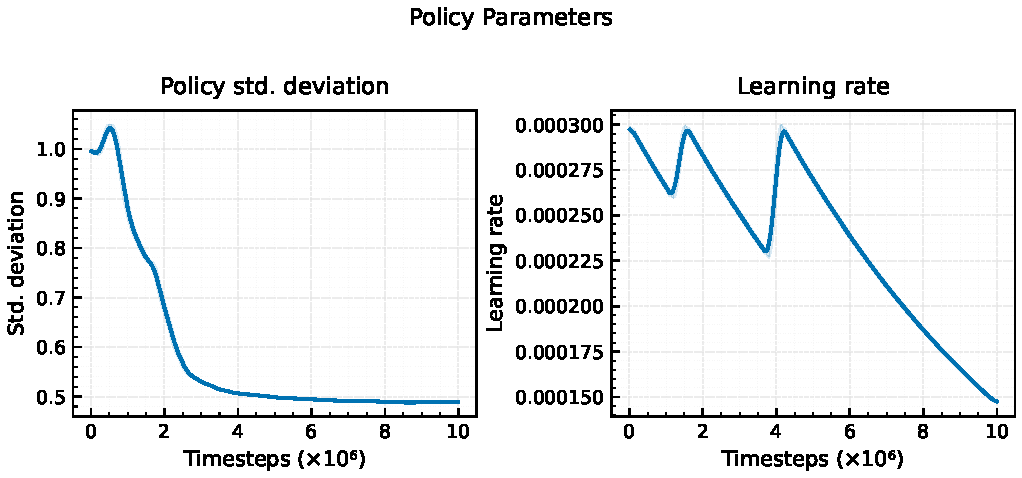
\includegraphics[width=1\textwidth]{images/chapter5/policy_parameters.pdf}
    \caption{The key policy parameters throughout training: the action standard deviation and the learning rate.}
    \label{fig:policy_parameters}
\end{figure}
\FloatBarrier

\subsection{PPO metrics}

\figurename~\ref{fig:ppo_diagnostic} reports three diagnostic metrics that characterise the quality of the policy updates and the critic's learning progress throughout training: the approximate KL divergence, the clip fraction, and the explained variance.

\subsubsection{Approximate KL divergence}
The approximate KL divergence measures how much the new policy has shifted from the old one following each gradient update, and serves as a key indicator of update stability. It is estimated as:

\begin{equation}
    \widehat{D}_{\mathrm{KL}} \approx \mathbb{E}_t \left[ \log \frac{\pi_{\theta_\mathrm{old}}(a_t | s_t)}{\pi_\theta(a_t | s_t)} \right]
\end{equation}
The approximate KL divergence begins at approximately $0.03$ at the start of training, decreases steadily, and increases to $0.03$ at the end of the run. The rapid decay and subsequent stability confirm that the clip range constraint ($\varepsilon = 0.2$) was effective in preventing excessively large policy updates. 

\subsubsection{Clip Fraction}
The clip fraction reports the proportion of samples in each rollout batch for which the probability ratio $r_t(\theta) = \pi_\theta(a_t | s_t) / \pi_{\theta_\mathrm{old}}(a_t|s_t)$ exceeded the clip boundary, i.e. fell outside the interval $[1 - \varepsilon,\,1]$. The clip fraction starts at approximately $0.2$ in the early stages of training and then increases, stabilising around $0.30$ for the rest of the run; The elevated values at the end suggests that the policy was undergoing substantial changes in the first updates, consistent with the high approximate KL divergence observed at the same time. As training progresses, the clip fraction settles into a healthy range, indicating that only a moderate proportion of samples were actively constrained by the clipping mechanism. 

\subsubsection{Explained Variance}
The explained variance quantifies how accurately the value function $V_\theta(s)$ predicts the empirical returns collected during rollouts:

\begin{equation}
    \mathrm{EV} = 1 - \frac{\mathrm{Var}(y - \hat{y})}{\mathrm{Var}(y)}
\end{equation}
where $y$ denotes the observed returns and $\hat{y}$ the value function predictions. A value of $1$ corresponds to perfect prediction, while values near $0$ or below indicate that the critic is no better than a constant baseline; The explained variance increases progressively towards $0.9$ over the course of training, demonstrating that the critic successfully learned to approximate the value landscape of the task.

\begin{figure}[htbp]
    \centering
    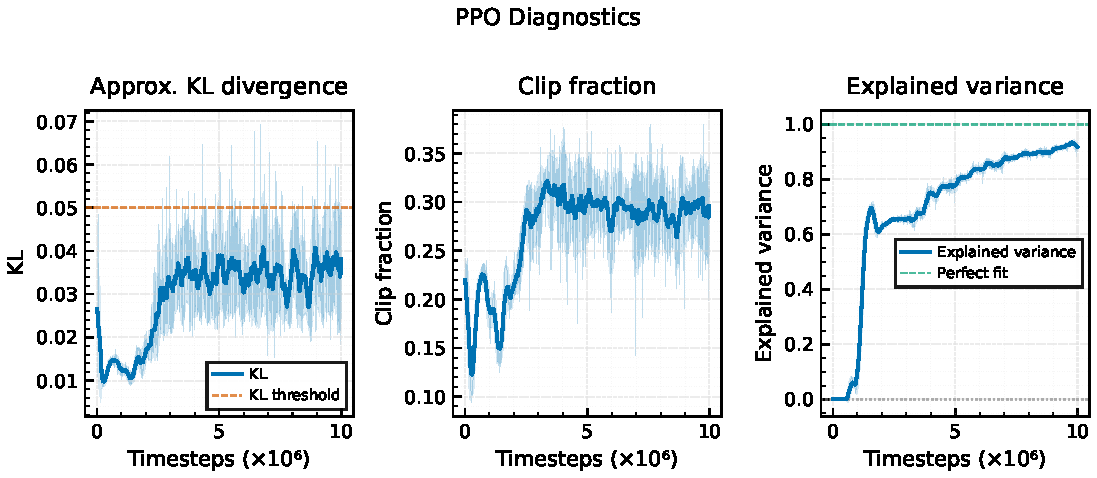
\includegraphics[width=1\textwidth]{images/chapter5/ppo_diagnostics.pdf}
    \caption{The three diagnostic metrics that characterise the quality of the policy updates and the critic's learning progress throughout training: the approximate KL divergence, the clip fraction, and the explained variance.}
    \label{fig:ppo_diagnostic}
\end{figure}
\FloatBarrier

\subsection{Training Convergence}

\figurename~\ref{fig:training_convergence} presents the two primary convergence indicators over the course of training: the mean episode reward and the valid-action rate. The reward curve (left axis) reflects how well the agent is optimising the beamforming objective, while the valid rate (right axis) measures the fraction of timesteps in which the agent produced a configuration that satisfied all amplitude and phase constraints. 

\begin{figure}[htbp]
    \centering
    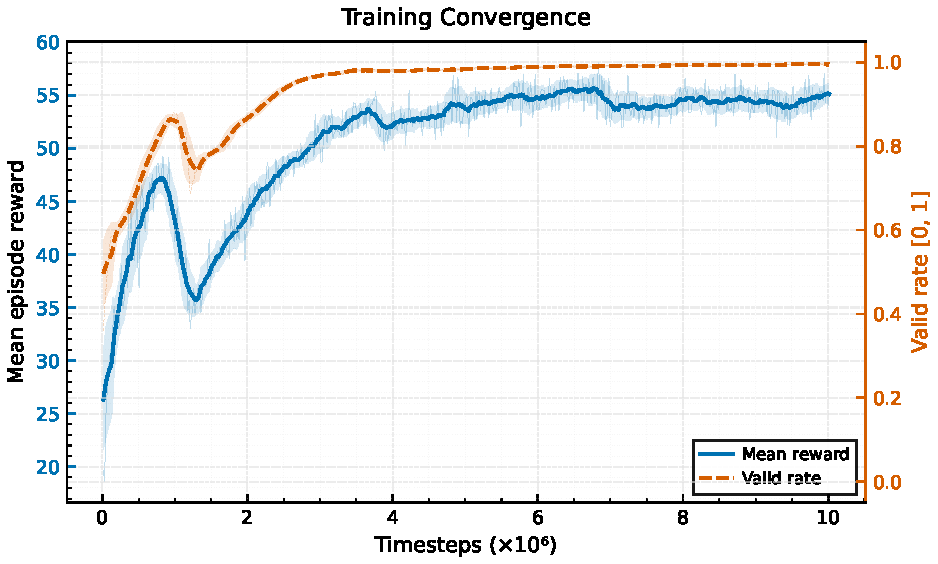
\includegraphics[width=0.80\textwidth]{images/chapter5/training_convergence.pdf}
    \caption{Training convergence: mean episode reward (left axis) and valid-action rate (right axis) over training timesteps.}
    \label{fig:training_convergence}
\end{figure}
\FloatBarrier

\subsection{Training losses}

\figurename~\ref{fig:training_losses} reports the four loss components optimised jointly by\gls{PPO} throughout training: the policy gradient loss, the value loss, the entropy loss, and the total combined loss. Monitoring these components is essential to distinguish between healthy optimisation dynamics and pathological behavior that may not be apparent from reward curves alone.

\subsubsection{Policy Gradient Loss}
The core actor loss measures how well the policy is being pushed toward higher-advantage actions. Under the clipped\gls{PPO} objective it is defined as:
\begin{equation}
    L^{\mathrm{PG}} = -\mathbb{E}_t \left[ \min \left( r_t(\theta)\hat{A}_t,\ \mathrm{clip}(r_t(\theta),\, 1 - \varepsilon,\, 1 + \varepsilon)\hat{A}_t \right) \right]
\end{equation}
where the negative sign arises because gradient descent is used to maximise expected reward. The clipping embedded in this objective is what distinguishes\gls{PPO} from vanilla policy gradient methods, and directly reflects whether policy updates are aligned with the advantage estimates~\cite{schulman2017ppo}. During healthy training this loss should remain small because large values indicate that updates are too aggressive.

\subsection{Value Loss}
The critic loss measures how accurately the value function predicts empirical returns, formulated as mean squared error between predicted state values and target returns:
\begin{equation}
    L^{\mathrm{VF}} = \mathbb{E}_t \left[ \left( V_\theta(s_t) - V_t^{\mathrm{target}} \right)^2 \right]
\end{equation}
This term is scaled by a coefficient $c_1$ before being added to the total loss, since an unscaled value loss would otherwise dominate the gradient signal. A higher value loss early in training is acceptable as long as it decreases as the critic learns since persistent high values would keep advantage estimates noisy and destabilise the actor.

\subsection{Entropy Loss}
The entropy loss measures the randomness of the policy's action distribution:

\begin{equation}
    L^{\mathrm{ENT}} = -\mathbb{E}_t \left[ H\!\left(\pi_\theta(\cdot \mid s_t)\right) \right] = \mathbb{E}_t \left[ \sum_a \pi_\theta(a \mid s_t) \log \pi_\theta(a \mid s_t) \right]
\end{equation}
A high-entropy policy is more exploratory, while a low-entropy policy is more deterministic. The entropy loss should gradually decrease over training as the policy becomes more confident.

\subsection{Total Loss}

All three components are combined into a single scalar objective minimized by the Adam optimizer at each gradient step:
\begin{equation}
    L^{\mathrm{TOTAL}} = L^{\mathrm{PG}} + c_1 \cdot L^{\mathrm{VF}} - c_2 \cdot L^{\mathrm{ENT}}
\end{equation}

As visualized in \figurename~\ref{fig:training_losses}, our losses behave in an ideal manner with values near $0$ at the end of the training.

\begin{figure}[htbp]
    \centering
    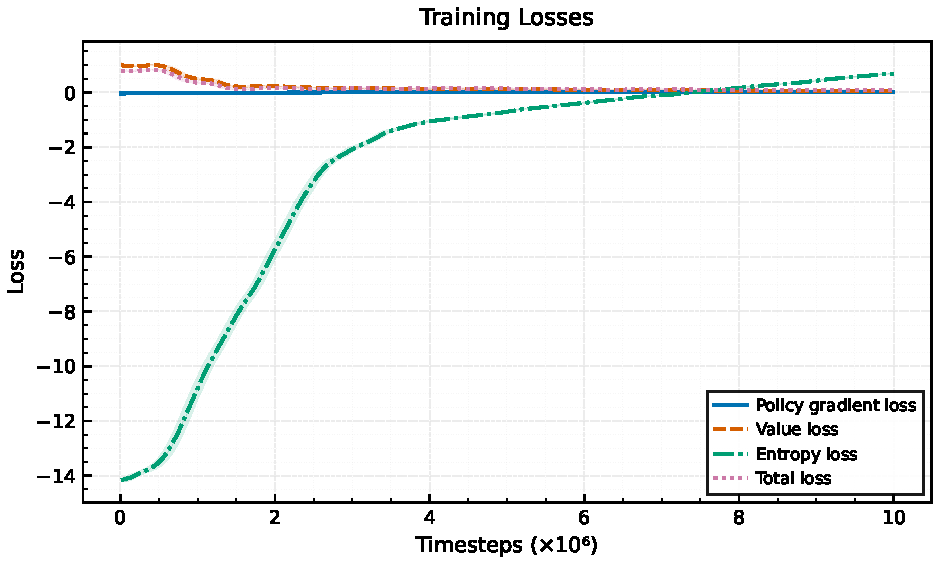
\includegraphics[width=0.85\textwidth]{images/chapter5/training_losses.pdf}
    \caption{The four loss components optimised jointly by\gls{PPO} throughout training: the policy gradient loss, the value loss, the entropy loss, and the total combined loss.}
    \label{fig:training_losses}
\end{figure}
\FloatBarrier

\subsection{Secrecy Performance}

\figurename~\ref{fig:secrecy_performance} tracks the\gls{BER} metrics throughout training on a logarithmic scale: the legitimate user\gls{BER}, the secrecy\gls{BER} and the minimum\gls{BER} of all possible eavesdropper angles. These curves reflect how well the agent is learning the physical-layer security objective: driving the legitimate\gls{BER} below the target threshold while maintaining a high eavesdropper\gls{BER}. 

\begin{figure}[htbp]
    \centering
    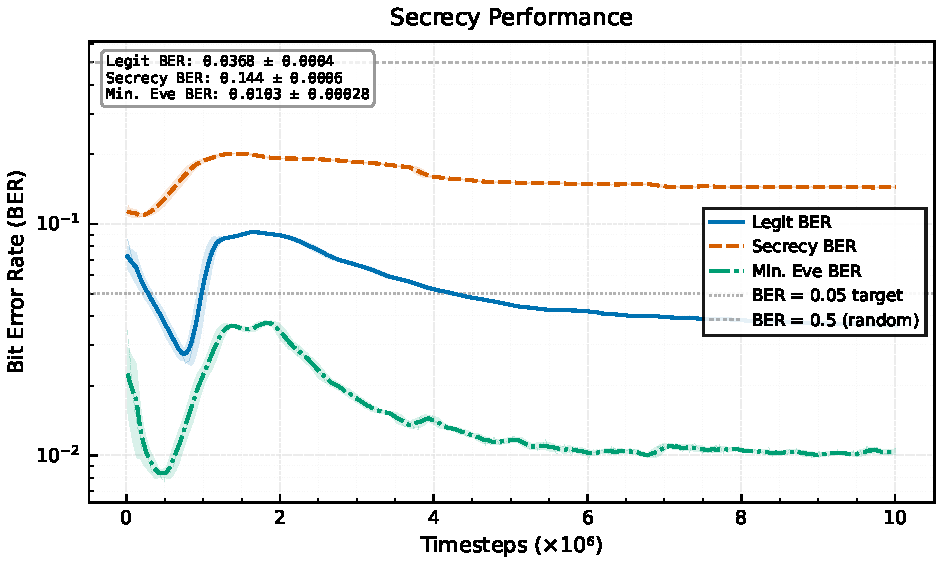
\includegraphics[width=0.75\textwidth]{images/chapter5/secrecy_performance.pdf}
    \caption{BER metrics throughout training: legitimate user\gls{BER}, secrecy\gls{BER}, and the minimum\gls{BER} of all possible eavesdropper angles on a logarithmic scale. Dashed reference lines at $\mathrm{BER}=0.05$ and $\mathrm{BER}=0.5$ are included for orientation.}
    \label{fig:secrecy_performance}
\end{figure}
\FloatBarrier
\subsection{Constraint Satisfaction}

\figurename~\ref{fig:constraint_satisfaction} shows the evolution of two constraint-related metrics during training: the valid-action rate and the fraction of eavesdropper directions with\gls{BER} below $0.1$. The valid rate measures how reliably the agent produces configurations that satisfy the amplitude floor and phase flatness constraints, while the low-BER fraction indicates how well the secrecy objective is met across the eavesdropper space.

\begin{figure}[htbp]
    \centering
    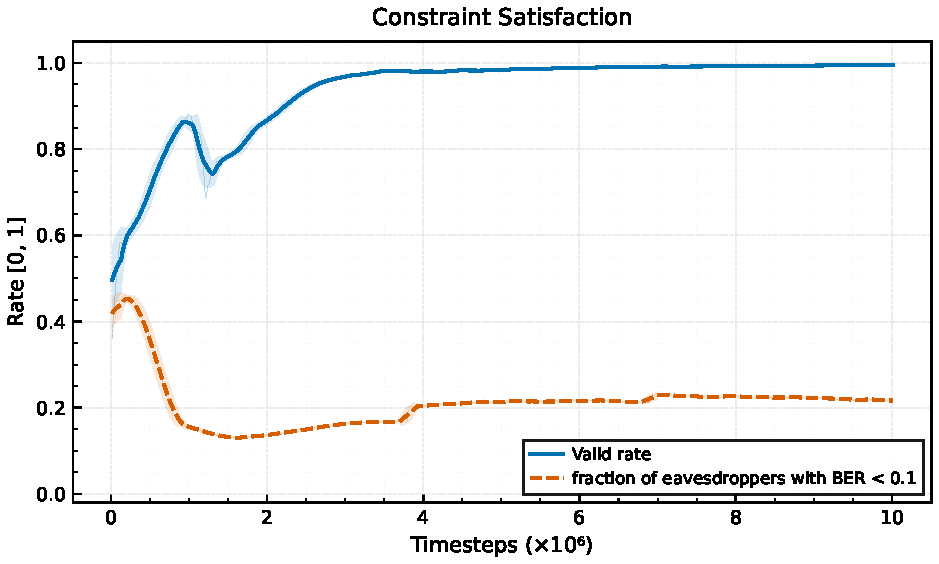
\includegraphics[width=0.80\textwidth]{images/chapter5/constraint_satisfaction.pdf}
    \caption{Constraint satisfaction throughout training: valid-action rate and fraction of eavesdropper directions with $\mathrm{BER} < 0.1$.}
    \label{fig:constraint_satisfaction}
\end{figure}
\FloatBarrier

\subsection{Training Overview}

\figurename~\ref{fig:training_overview} provides a concise four-panel summary of key training metrics: mean episode reward, valid-action rate, legitimate user\gls{BER}. and secrecy\gls{BER}.

\begin{figure}[htbp]
    \centering
    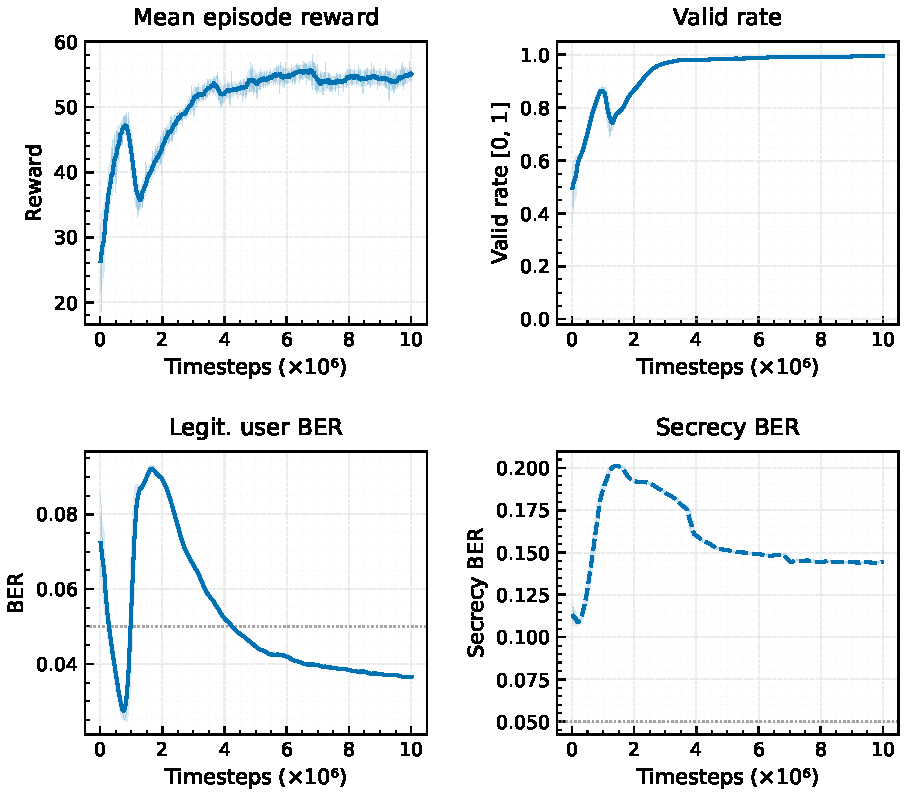
\includegraphics[width=1\textwidth]{images/chapter5/overview.pdf}
    \caption{Four-panel training overview: mean episode reward, valid-action rate, legitimate user\gls{BER}, and secrecy\gls{BER}.}
    \label{fig:training_overview}
\end{figure}
\FloatBarrier

%**************************************************************
\section{Inference results}
\subsubsection{Beam pattern}

\figurename~\ref{fig:model_beam_pattern} presents the beam patterns obtained at inference for three representative target angles: $\varphi^* \in \{-60\degree, 0\degree, 60\degree\}$, as described in the plot legend. In each case the solid line corresponds to the deterministic solution (\texttt{deterministic=True}), representing the policy mean $\mu_\theta(\varphi^*)$. All three deterministic beams exhibit a well-defined principal lobe with its peak precisely aligned to the desired angle, confirming that the policy has learned to map each target direction to a valid, high-quality beamforming configuration. \\
The transparent lines of matching color represent stochastic samples drawn from the same policy (\texttt{deterministic=False}). These samples preserve the correct pointing direction, their principal lobe peaks remain at $\varphi^*$ while exhibiting moderate sidelobe energy relative to the deterministic solution. Importantly, the amplitude loss at the main lobe is negligible across all stochastic samples, confirming that diversity is achieved without compromising the primary beamforming objective.

\begin{figure}[htbp]
    \centering
    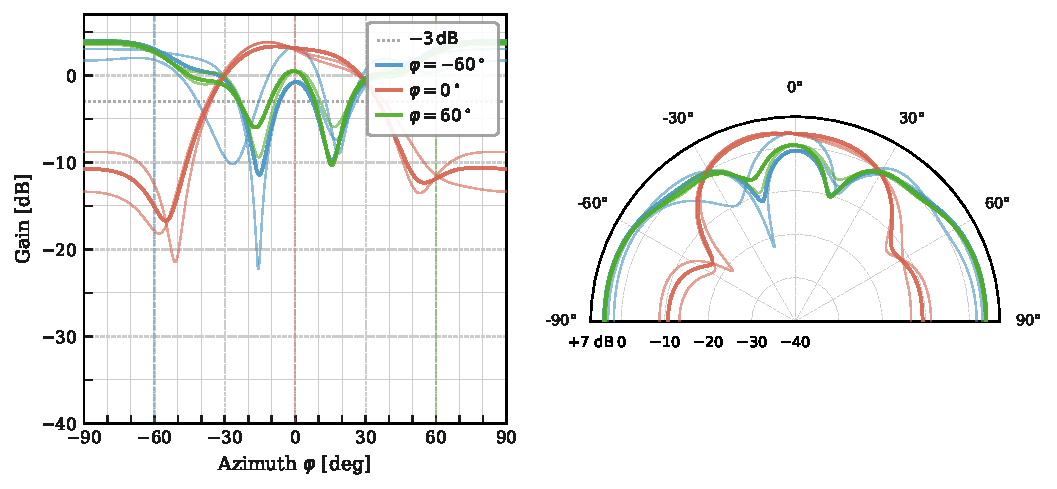
\includegraphics[width=1\textwidth]{images/chapter5/beam_pattern.pdf}
    \caption{Beam patterns produced by the trained\gls{PPO} agent for three target angles ($\varphi = -60\degree$, $0\degree$, $60\degree$). Solid lines show deterministic inference; transparent lines show stochastic samples.}
    \label{fig:model_beam_pattern}
\end{figure}
\FloatBarrier

\subsubsection{Diversity Analysis}
\label{sec:diversity_analysis}
\figurename~\ref{fig:model_diversity_analysis} reports the outcome of 100 stochastic inference draws at each integer target angle $\varphi^* \in [-90\degree, 90\degree]$, for a total of 18{,}100 samples. Each bar is decomposed into three categories: unique valid configurations (blue), duplicate solutions, and failed configurations that violated the amplitude or phase constraints (red). \\
The results confirm the robustness of the trained policy across the full angular range. Of all samples, 18{,}072 (99.8\%) are unique valid configurations, 27 (0.1\%) are duplicates, and only 1 (0.0\%) is a failure, demonstrating that the policy reliably explores distinct regions of the solution manifold rather than collapsing onto a single solution. \\
The sole systematic deviation from perfect diversity is a mild concentration of duplicate samples in the broadside region ($\varphi^* \in [-9\degree, 9\degree]$). Outside this region, duplicates are negligible and failures are absent across the entire angular range.

\begin{figure}[htbp]
    \centering
    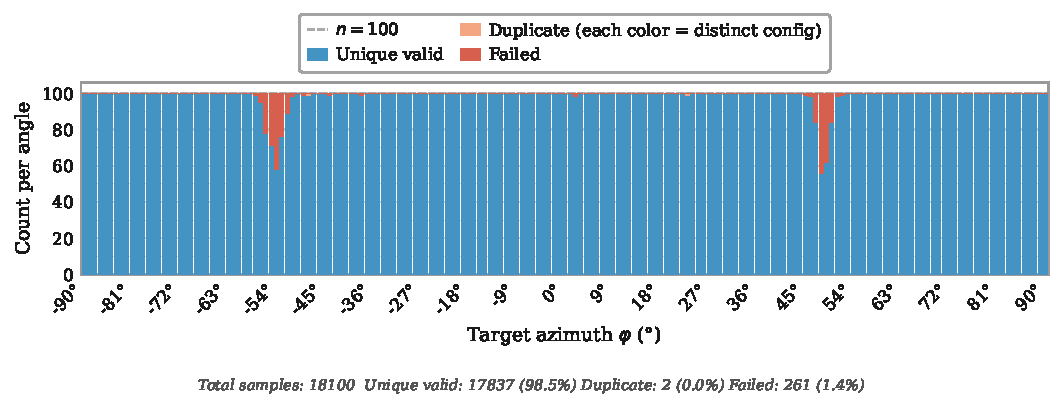
\includegraphics[width=1\textwidth]{images/chapter5/diversity_analysis.pdf}
    \caption{Outcome of 100 stochastic inference draws at each integer target angle $\varphi^* \in [-90\degree, 90\degree]$, for a total of 18{,}100 samples. Each bar is decomposed into three categories: unique valid configurations (blue), duplicate solutions (orange), and failed configurations that violated the amplitude or phase constraints (red).}
    \label{fig:model_diversity_analysis}
\end{figure}
\FloatBarrier

\subsubsection{Bit Error Rate \& Symbol Error Rate}

\figurename~\ref{fig:model_ber_ser_ebn0} presents the\gls{SER} and\gls{BER} curves obtained for $M$-\gls{PSK} modulation orders $M \in \{2, 4, 8, 16\}$, at target angle $\varphi = 30\degree$ with a $N = 5$ element\gls{ULA}. For each modulation order, $K = 5$ stochastic beamforming configurations are sampled from the trained policy, producing the thin solid curves, whose spread directly reflects the diversity of valid solutions explored by the agent. The dashed curves represent the theoretical baseline assuming a perfect array gain equal to $N$, serving as an upper bound on achievable performance.\\
Two observations are immediate. First, the simulated curves are consistently shifted to the right of their theoretical counterparts across all modulation orders; This gap is a direct consequence of the stochastic beamforming policy: unlike a deterministic matched filter, the sampled configurations do not maximize array gain at every draw, instead trading peak performance for solution diversity and secrecy. Second, the spread among the $K=5$ curves per modulation order is non-negligible, particularly for higher $M$, confirming that distinct stochastic samples produce meaningfully different received $E_b/N_0$ conditions.\\
These results should be interpreted in the context of the present work's primary objective. The proposed framework is not intended as a production-ready beamformer optimized for link budget, but as a foundational demonstration that a\gls{RL} agent can learn to navigate the directional modulation solution manifold and produce valid, diverse configurations.

\begin{figure}[htbp]
    \centering
    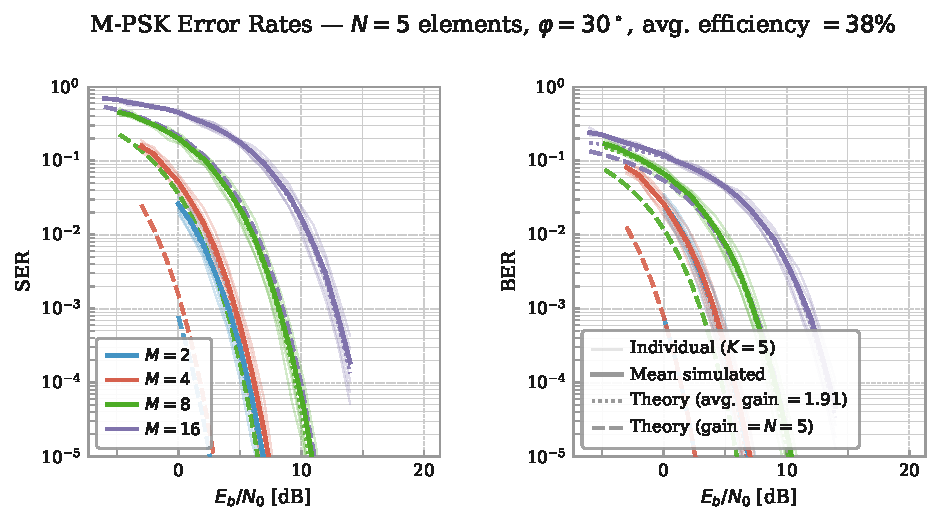
\includegraphics[width=1\textwidth]{images/chapter5/ber_ser_ebn0.pdf}
    \caption{\gls{SER} and\gls{BER} curves obtained for $M$-\gls{PSK} modulation orders $M \in \{2, 4, 8, 16\}$, at target angle $\varphi = 30\degree$ with a $N = 5$ element\gls{ULA}.}
    \label{fig:model_ber_ser_ebn0}
\end{figure}
\FloatBarrier



\subsubsection{Constellation}

\figurename~\ref{fig:model_constellations} illustrate the relationship between array gain, modulation order, and noise margin. Symbol error rates are estimated over 50,000 Monte Carlo trials per modulation scheme.
At $M = 2$ (BPSK), performance is near-perfect: the two symbol clouds are well-separated and entirely contained within their respective decision regions, yielding\gls{BER} $= 0.000$. The system operates comfortably above the noise floor despite the sub-ideal array gain, confirming that BPSK is robust to the gain loss introduced by stochastic beamforming. At $M = 4$ (QPSK), the constellation remains largely correct, with only isolated error points visible near decision boundaries, indicating that the inter-symbol distance is still sufficient at this SNR.
The picture degrades substantially at $M = 8$, where the reduced angular separation between symbols ($45\degree$) brings the noise clouds into contact with adjacent decision regions, producing a\gls{BER} of $1.4 \times 10^{-2}$. While individual symbol clusters are still discernible, a non-negligible fraction of received points cross decision boundaries, particularly for symbols in close angular proximity. At $M = 16$, the system experiences catastrophic failure (SER $= 2.1\times10^{-1}$): the $22.5\degree$ inter-symbol spacing is irreconcilable with the noise variance induced by the limited array gain, and the received point cloud is almost uniformly distributed across decision regions, rendering reliable demodulation impossible at this SNR.\\
These results establish a clear operating boundary for the proposed beamforming framework: modulation orders up to $M = 4$ are reliably supported at $E_s/N_0 = 10$~dB given the current array configuration and gain efficiency. Higher-order modulation would require either a larger array to recover gain, a higher operating SNR, or improvements on the gain-aware reward signal during training to steer the policy toward configurations that better preserve array gain.

\begin{figure}[htbp]
    \centering
    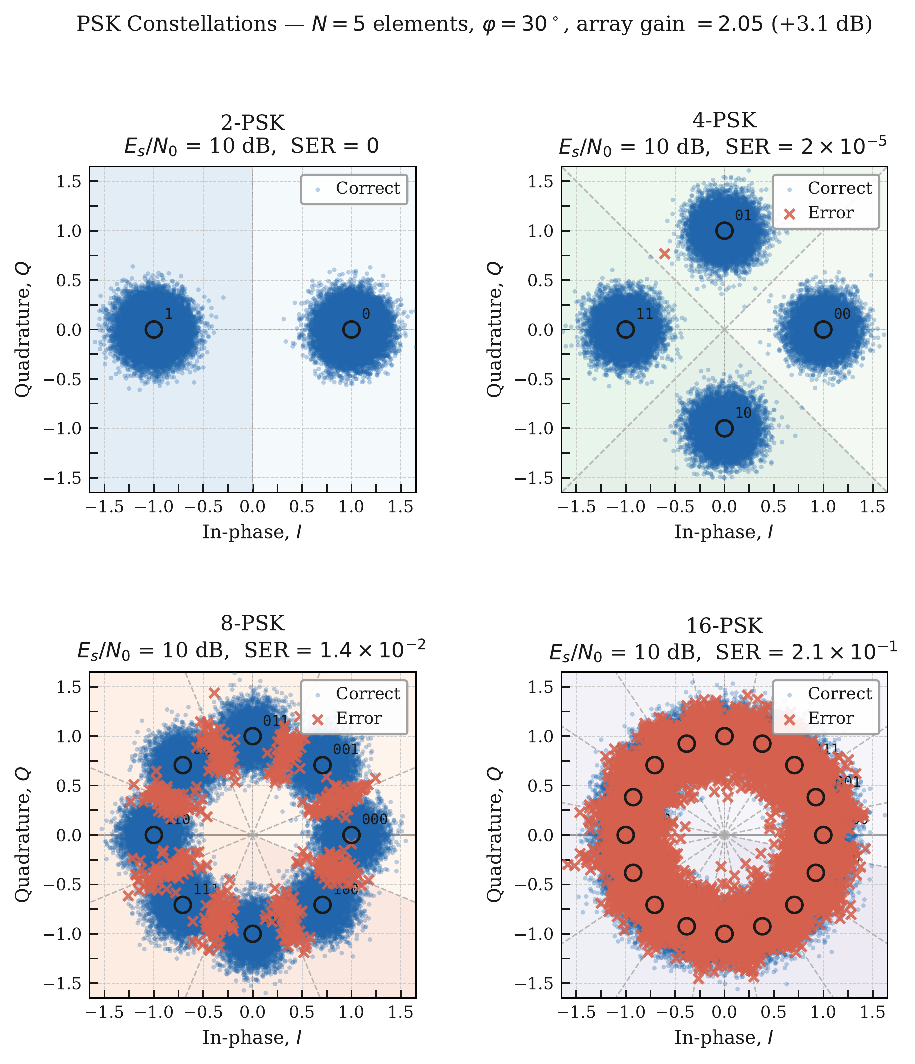
\includegraphics[width=1\textwidth]{images/chapter5/constellations.pdf}
    \caption{IQ constellations for $M$-PSK modulation at $E_s/N_0 = 10$~dB with $N=5$ elements at $\varphi = 30\degree$. Blue dots indicate correct detections; red crosses indicate symbol errors. Open circles mark ideal symbol positions with Gray-coded bit labels.}
    \label{fig:model_constellations}
\end{figure}
\FloatBarrier

\subsubsection{SER vs.\ Angle}

\figurename~\ref{fig:ser_vs_angle} shows the\gls{SER} as a function of azimuth angle at a fixed $E_s/N_0 = 10$~dB, with the legitimate user steered to $\varphi = 30\degree$. A well-trained beamforming policy should maintain low error rates in the targeted direction while exhibiting high error rates elsewhere, indicating signal distortion outside the intended direction. In our plot it can be observed that the best angle for eavesdroppers are those that are physically near the legittimate receiver and the further away the eavesdropper is, the greater the error rate.

\begin{figure}[htbp]
    \centering
    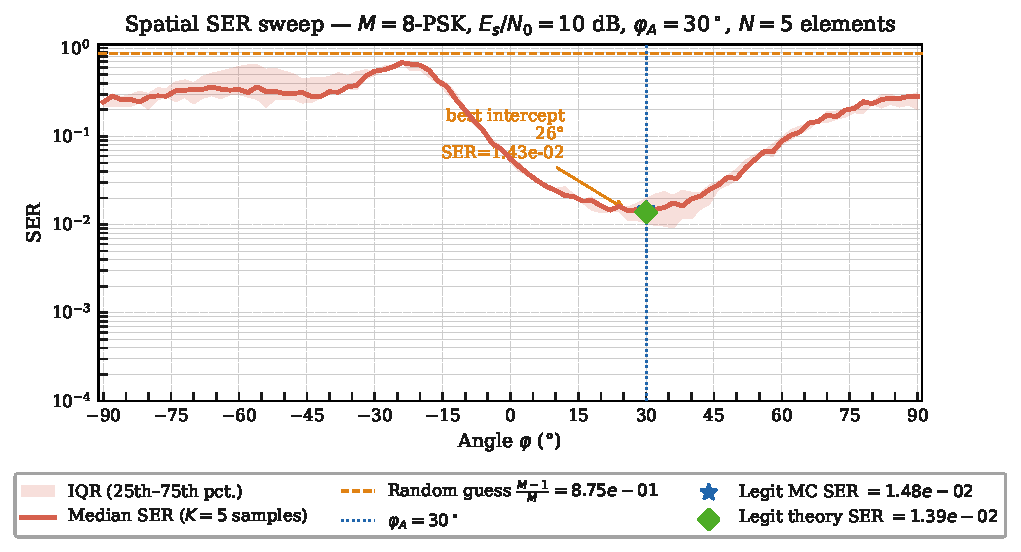
\includegraphics[width=1\textwidth]{images/chapter5/ser_vs_angle.pdf}
    \caption{SER as a function of azimuth angle at fixed $E_s/N_0 = 10$~dB, with the legitimate user steered to $\varphi = 30\degree$.}
    \label{fig:ser_vs_angle}
\end{figure}
\FloatBarrier

\figurename~\ref{fig:secrecy_matrix} presents a more generalized view of the physical-layer security: the secrecy matrix obtained by evaluating the\gls{BER} over a grid of legitimate and eavesdropper angles at fixed $E_s/N_0 = 10$~dB. For each pair $(\varphi_\mathrm{Bob}, \varphi_\mathrm{Eve})$, the matrix reports the channel secrecy of the configuration. It can be observed that, as shown along the center diagonal, the closer the eavesdropper is to the target angle the lower the channel secrecy.

\begin{figure}[htbp]
    \centering
    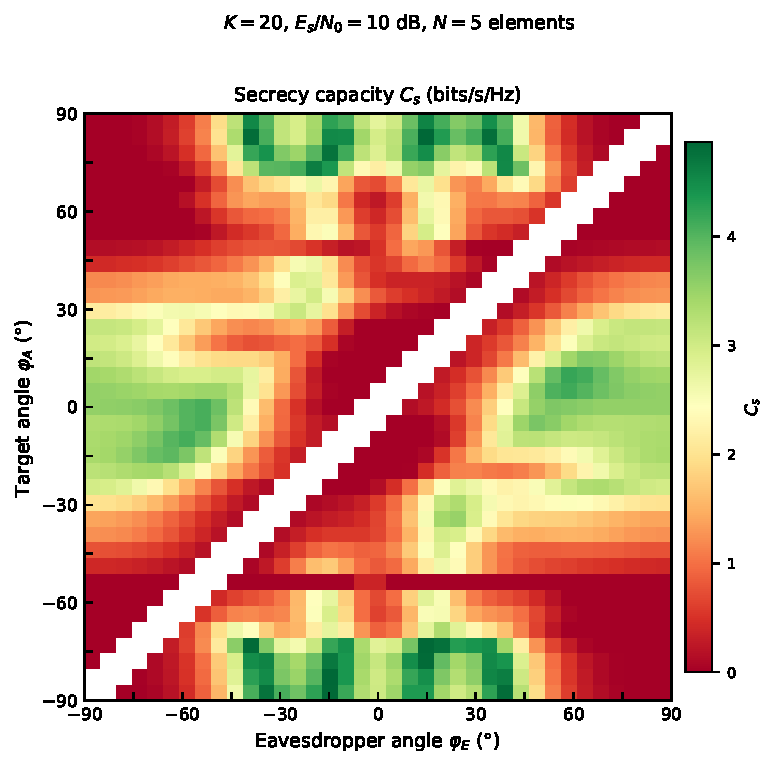
\includegraphics[width=1\textwidth]{images/chapter5/secrecy_matrix.pdf}
    \caption{Secrecy matrix:\gls{BER} evaluated over a grid of legitimate-user and eavesdropper angles at fixed $E_s/N_0 = 10$~dB.}
    \label{fig:secrecy_matrix}
\end{figure}
\FloatBarrier

\subsubsection{Amplitude Profile}

\figurename~\ref{fig:amplitude_profile} illustrates the amplitude weights of the antenna elements produced by the trained policy throughout the full angular range $\varphi \in [-90\degree, 90\degree]$. For each target angle, $K = 5$ stochastic samples are drawn from the policy and the resulting amplitude profiles are superimposed. This figure reveals how the agent allocates power across the array elements as a function of steering direction, revealing that near angles in which the phase constraints become harder to satisfy (\subsectionname~\ref{subsec:angle_dependant_constraint}) the model will allocate less amplitude or none at all to specific elements in order to reduce the complexity.

\begin{figure}[htbp]
    \centering
    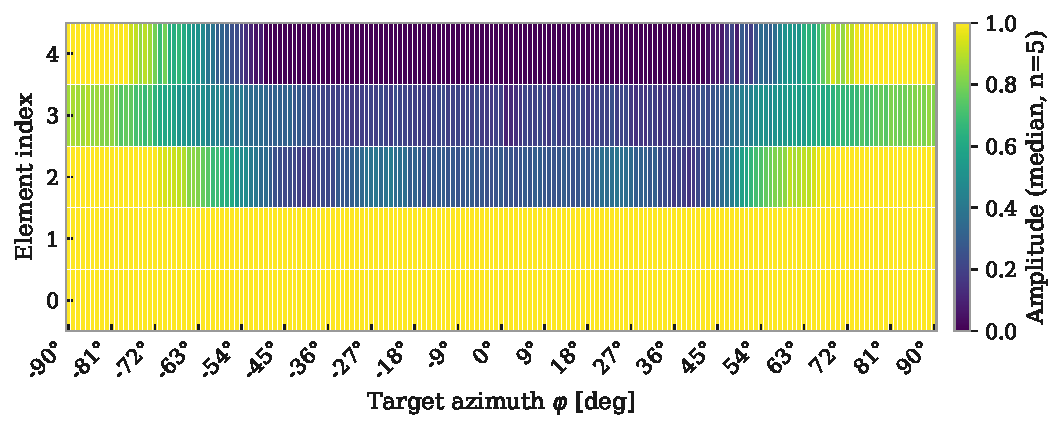
\includegraphics[width=1\textwidth]{images/chapter5/amplitude_profile.pdf}
    \caption{Antenna element amplitude weights produced by the trained\gls{PPO} policy across target angles $\varphi \in [-90\degree, 90\degree]$, with $K=5$ stochastic samples per angle.}
    \label{fig:amplitude_profile}
\end{figure}
\FloatBarrier

%**************************************************************
\section{Comparison with Random Search}
\label{sec:benchmark}

This section benchmarks the trained\gls{PPO} model against a two baselines:
\begin{itemize}
    \item a naive random phase search;
    \item\gls{CEM}, a population-based stochastic optimization approach.
\end{itemize}
For each azimuth angle $\varphi \in [-90\degree, 90\degree]$, all three methods are tasked with finding a valid beamforming configuration that satisfies the amplitude floor and phase flatness constraints used during training. The random search draws uniform random phases from $[0, 2\pi)^N$ until a valid configuration is found or a maximum of $10{,}000$ attempts is exhausted;\gls{CEM} iteratively refines a sampling distribution over phase configurations by fitting to the best-performing samples from each generation, validating candidates as they are drawn; the\gls{PPO} model draws stochastic samples from the trained policy and validates each one in turn, stopping at the first valid draw or after $500$ attempts.

\subsection{Sample Efficiency}

\figurename~\ref{fig:benchmark_efficiency} compares the three methods in terms of the number of candidates evaluated before a valid solution is found (left panel) and the success rate across angles (right panel). Solid lines report the median number of tries, with shaded bands covering the 25th--75th percentile range across independent repetitions. The\gls{PPO} model requires substantially fewer candidates to find a valid configuration at most angles.\gls{CEM} improves on naive random search by adapting its sampling distribution over successive generations, but still requires considerably more candidates as it lacks any prior knowledge of the constraint structure. The naive random approach takes the shape of a gaussian distribution with the broadside angles requiring more tries, a trend similar to\gls{CEM} sice it is initialized from a similarly uniformed distribution.
\begin{figure}[htbp]
    \centering
    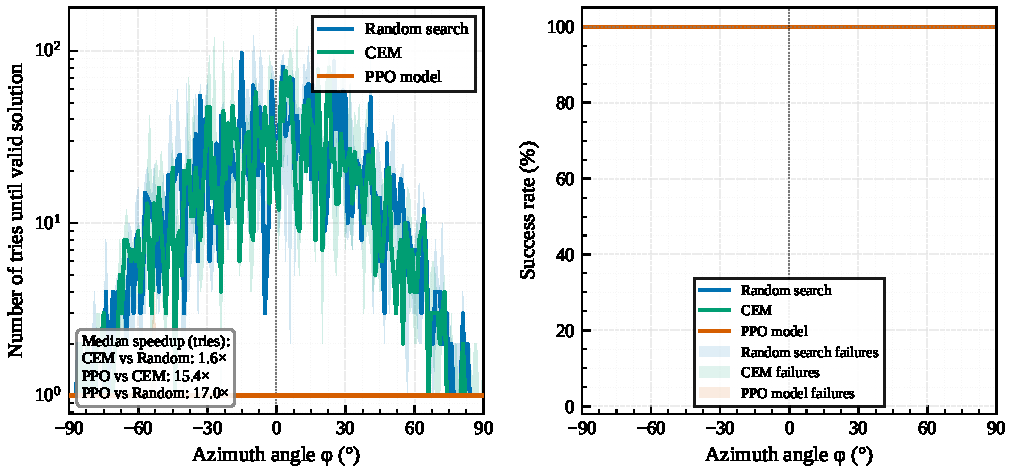
\includegraphics[width=0.8\textwidth]{images/chapter5/benchmark_efficiency.pdf}
    \caption{Sample efficiency comparison between\gls{PPO} model,\gls{CEM}, and random search: number of tries to find a valid configuration (left) and success rate across angles (right). Shaded bands show the 25th-75th percentile range.}
    \label{fig:benchmark_efficiency}
\end{figure}
\FloatBarrier

\subsection{Search Latency}

\figurename~\ref{fig:benchmark_latency} reports the total wall-clock latency (in milliseconds) required to find a valid beamforming configuration for each azimuth angle. The median latency annotations in the figure quantify the practical speed advantage of the learned policy over both baselines: the median latency is $0.3ms$ for the learned policy, $0.7ms$ for\gls{CEM} and $2.1ms$ for random search. These results indicate that, altough\gls{CEM}'s adaptive sampling offers a modest efficiency gain over a purely random strategy, it does not approach the latency reduction afforded by the learned policy.
\\
\\
It is worth noting that this comparison, while informative of raw search efficiency, is not entirely like-for-like: random search and\gls{CEM} are only tasked with satisfying the amplitude floor and phase flatness constraints, whereas the\gls{PPO} model is trained under an objective that additionally rewards configurations which degrade the\gls{SNR} at potential eavesdropper locations. The speedup and sample efficiency gains reported above therefore likely understate the relative advantage of the learned policy, which must satisfy a strictly harder, multi-objective problem within the same or fewer search attempts.

\begin{figure}[htbp]
    \centering
    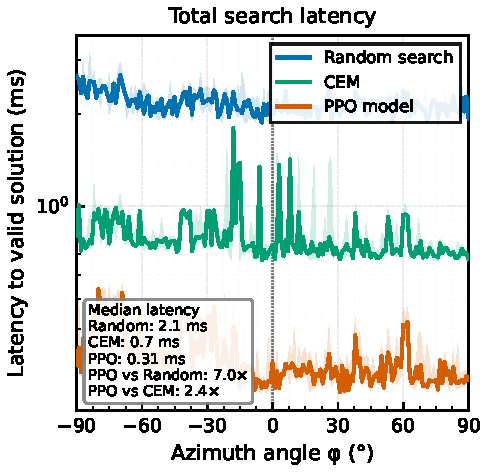
\includegraphics[width=0.6\textwidth]{images/chapter5/benchmark_latency.pdf}
    \caption{Total latency (ms) to find a valid beamforming configuration:\gls{PPO} model vs.\\gls{CEM} vs.\ random search across all azimuth angles. Shaded bands show the 25th--75th percentile range.}
    \label{fig:benchmark_latency}
\end{figure}
\FloatBarrier

\section{Training variation}

The three experiments presented in this section explore modifications to the baseline $N=5$ system:
\begin{enumerate}
    \item flattens the curriculum, making the model face the final constraints from the very beginning;
    \item replaces the raw phase parameterisation with a physics-informed action parameterisation;
    \item builds on the second experiment by also scaling the array to $N=8$ elements.
\end{enumerate}

\subsection{Curriculum Learning flattened}
\label{subsec:curriculum_flattened}
\subsubsection{Results}

Removing the curriculum-learning stages and training directly under the full set of constraints leads to a clear degradation in performance: the learned policy fails to exploit the amplitude degrees of freedom available to the array and instead converges to solutions where nearly all antenna elements operate at maximum amplitude. In contrast to the curriculum-trained model, no meaningful power allocation strategy emerges, indicating that the optimisation problem becomes substantially harder when the agent is exposed to the complete constraint set from the beginning of training. This behaviour has a direct impact on secrecy performance, rendering the policy unable to learn to selectively attenuate individual elements, losing one of the few mechanisms available for shaping the array response beyond the constrained phase parameterisation. As a result, secrecy is largely neglected during optimisation and the resulting solutions exhibit significantly poorer secrecy characteristics than those obtained with the staged curriculum approach.
\\
\\
Analysis of 100 stochastic inference draws shows that the flattened-curriculum model produces consistently worse validation performance and completely fails for several receiver positions where the curriculum-trained policy remains robust. It can also be observed that the standard deviation of the validation metric remains higher throughout training and increases towards the final stages. Although the flattened-curriculum model ultimately converges to a valid policy, the final solution is markedly less stable, generalises poorly, and achieves substantially worse overall performance than the curriculum-based approach.

\begin{figure}[p]  % Force to its own page
    \centering
    \begin{subfigure}{\textwidth}
        \centering
        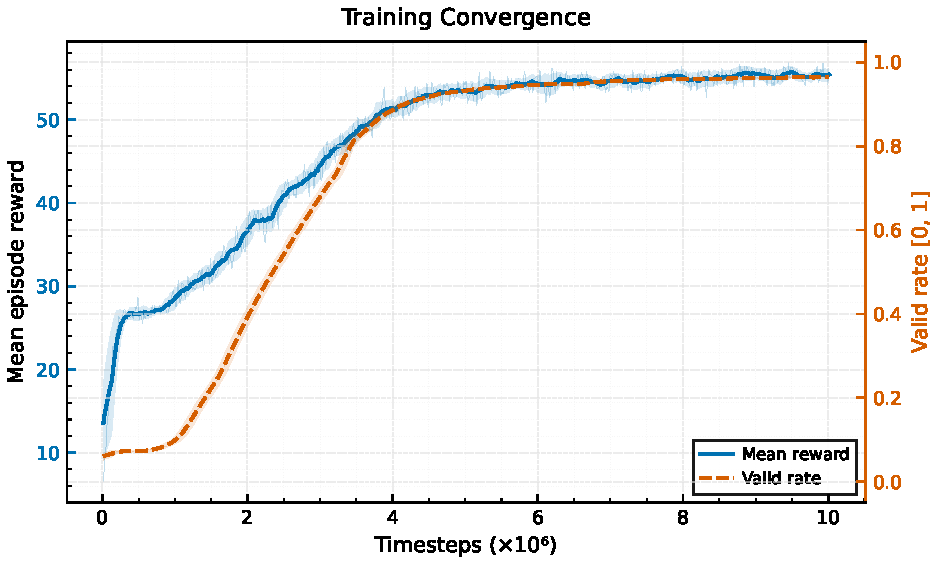
\includegraphics[width=0.8\textwidth]{images/chapter5/no_curriculum/training_convergence.pdf}
        \caption{Mean episode reward and valid-action rate}
        \label{fig:no_curriculum_training_convergence}
    \end{subfigure}
    
    \vspace{5pt}
    
    \begin{subfigure}{\textwidth}
        \centering
        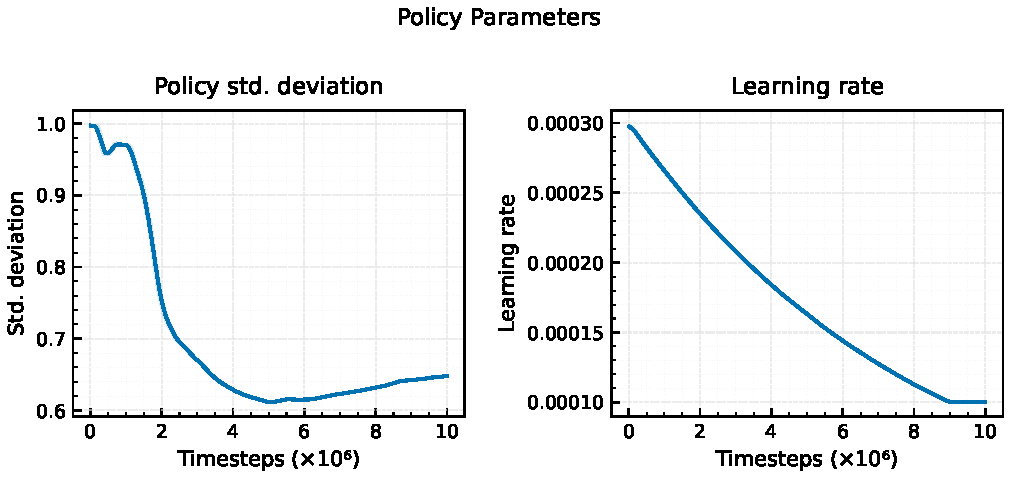
\includegraphics[width=0.8\textwidth]{images/chapter5/no_curriculum/policy_parameters.pdf}
        \caption{Action standard deviation and learning rate}
        \label{fig:no_curriculum_training_params}
    \end{subfigure}
    
    \vspace{5pt}
    
    \begin{subfigure}{\textwidth}
        \centering
        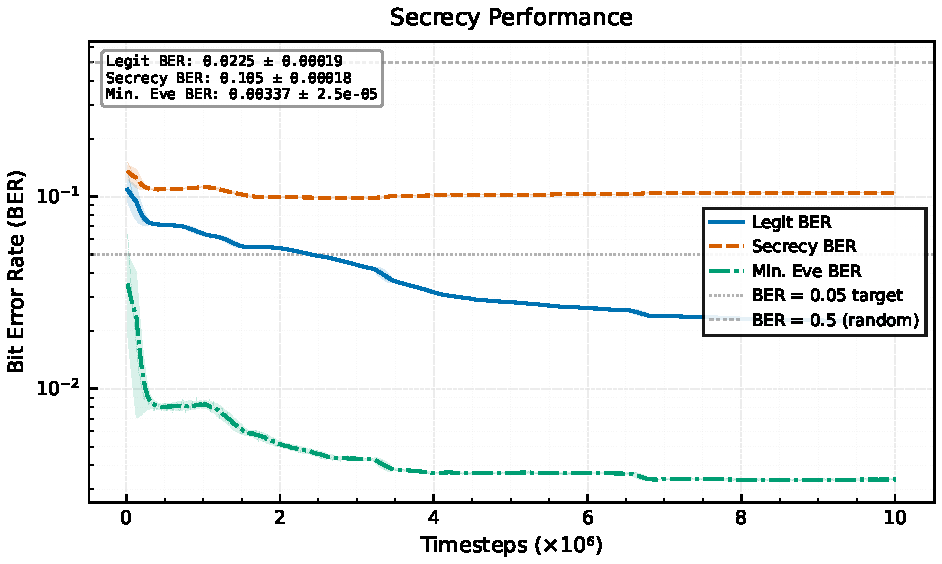
\includegraphics[width=0.8\textwidth]{images/chapter5/no_curriculum/secrecy_performance.pdf}
        \caption{BER metrics (legitimate user, secrecy, and minimum eavesdropper)}
        \label{fig:no_curriculum_training_ber}
    \end{subfigure}
    
    \caption{Training overview for the curriculum flattened $N=5$\gls{ULA}. Top: mean episode reward and valid-action rate. Middle: action standard deviation and learning rate. Bottom:\gls{BER} metrics (legitimate user, secrecy, and minimum eavesdropper).}
    \label{fig:no_curriculum_training}
\end{figure}

\begin{figure}[htbp]
    \centering
    \begin{minipage}[t]{0.49\textwidth}
        \centering
        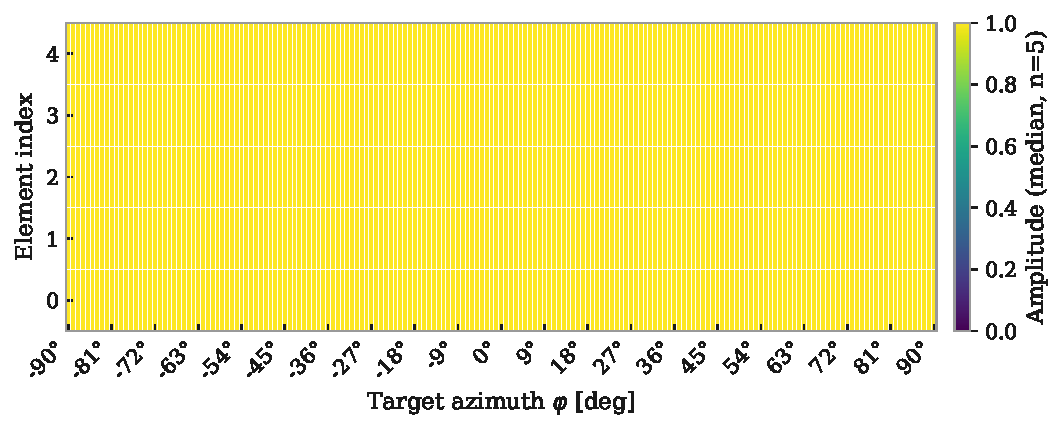
\includegraphics[width=\linewidth]{images/chapter5/no_curriculum/amplitude_profile.pdf}
    \end{minipage}\hfill
    \begin{minipage}[t]{0.49\textwidth}
        \centering
        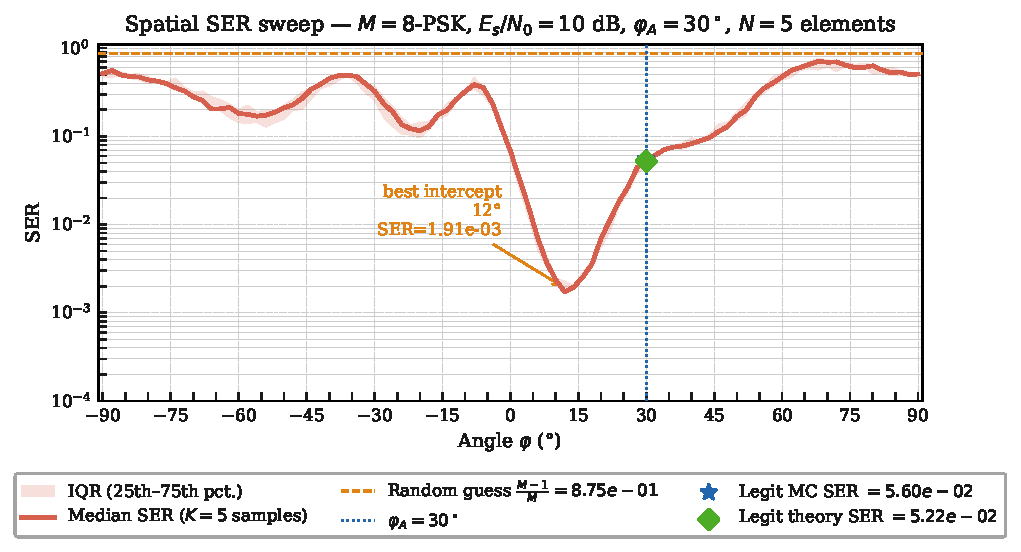
\includegraphics[width=\linewidth]{images/chapter5/no_curriculum/ser_vs_angle.pdf}
    \end{minipage}\\[4pt]
    \begin{minipage}[t]{0.49\textwidth}
        \centering
        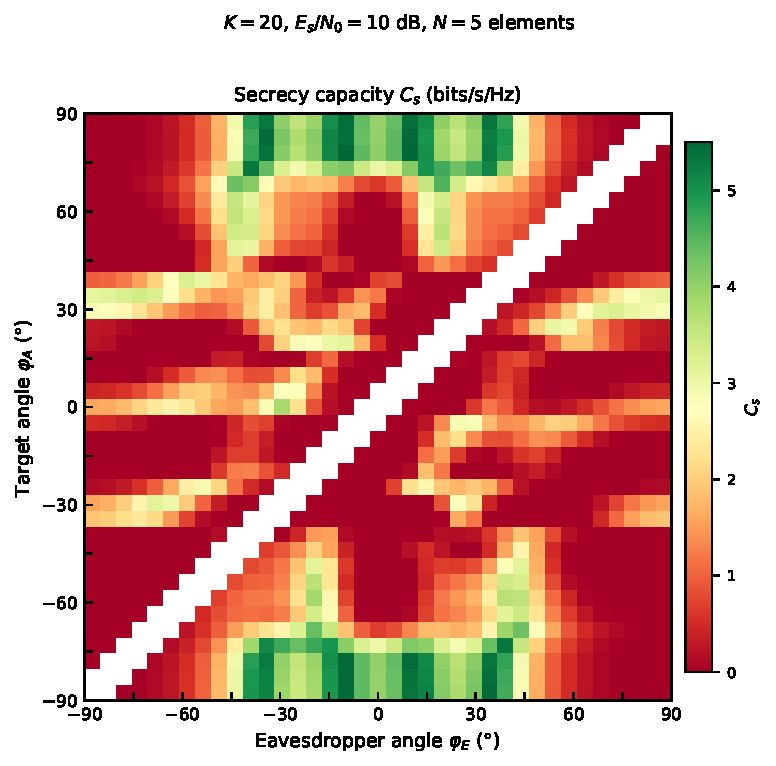
\includegraphics[width=\linewidth]{images/chapter5/no_curriculum/secrecy_matrix.pdf}
    \end{minipage}\hfill
    \begin{minipage}[t]{0.49\textwidth}
        \centering
        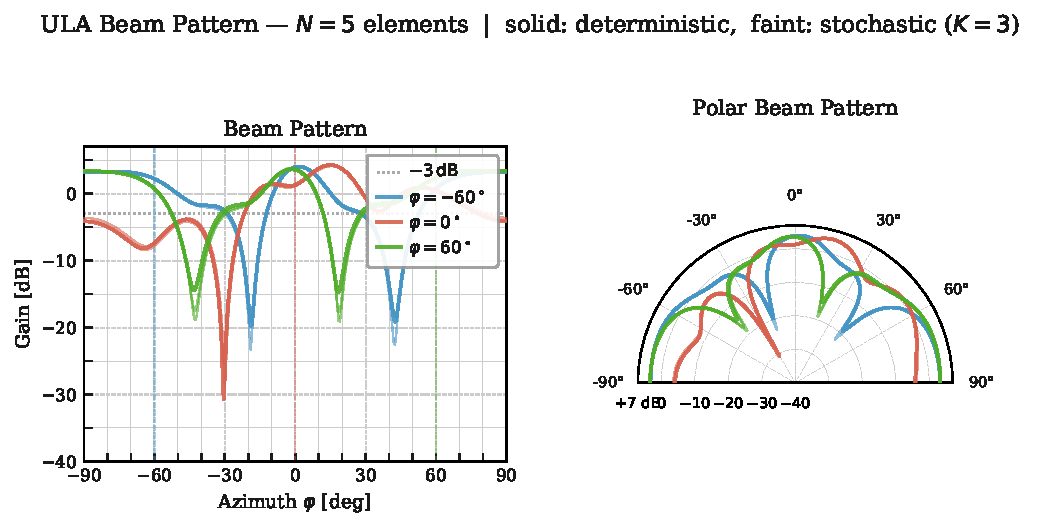
\includegraphics[width=\linewidth]{images/chapter5/no_curriculum/beam_pattern.pdf}
    \end{minipage}
    \caption{Inference overview for the curriculum flattened $N=5$\gls{ULA}. Top-left: amplitude profile across the full angular range.. Top-right:\gls{BER} vs.\ azimuth angle at $E_s/N_0 = 10$\,dB with the legitimate user at $\varphi = 30\degree$. Bottom-left: secrecy matrix. Bottom-right: beam patterns for $\varphi \in \{-60\degree, 0\degree, 60\degree\}$}
    \label{fig:no_curriculum_inference}
\end{figure}

\begin{figure}[htbp]
    \centering
    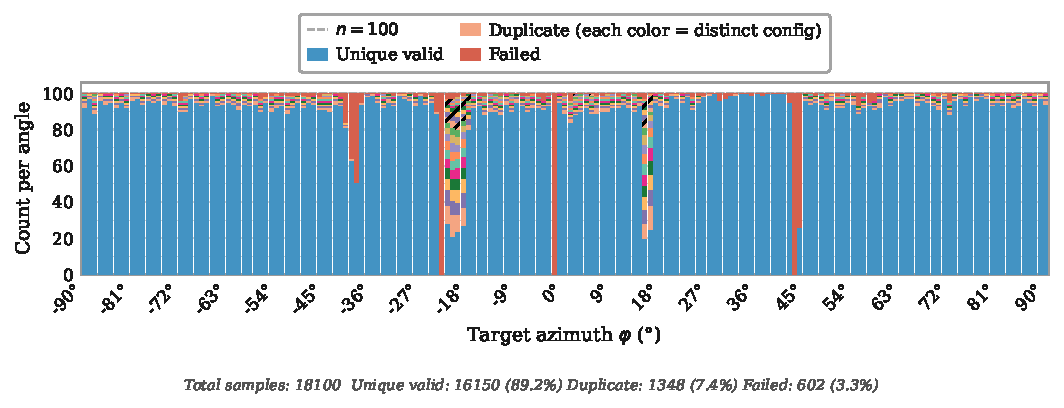
\includegraphics[width=1.0\textwidth]{images/chapter5/no_curriculum/diversity_analysis.pdf}
    \caption{Outcome of 100 stochastic inference draws at each integer target angle $\varphi^* \in [-90\degree, 90\degree]$, for a total of 18{,}100 samples for curriculum flattened model with\gls{ULA} with $N=5$ elements. Each bar is decomposed into three categories: unique valid configurations (blue), duplicate solutions, and failed configurations that violated the amplitude or phase constraints (red).}
    \label{fig:no_curriculum_diversity_analysis}
\end{figure}
\FloatBarrier

\subsection{Physics-informed action parameterisation}

\label{subsec:physics_informed}

In the baseline formulation the agent outputs $N$ independent phase values mapped uniformly to $[0, 2\pi)$, requiring it to discover solutions through reward signal alone. The physics-informed action parameterisation removes this burden by embedding the known analytical solution directly into the action decoder. For a\gls{ULA} with elements along the $y$-axis at spacing $d$, the optimal phase increment per element for steering to azimuth $\varphi$ is:
\begin{equation}
    \Delta\varphi = \frac{2\pi}{\lambda}\,d\,\sin\varphi
\end{equation}
Instead of predicting the $N$ phases directly, the agent predicts corrections on top of this:
\begin{equation}
    \varphi_n = n\!\left(\Delta\varphi + a_0\,\sigma_s\right) + a_n\,\sigma_p \qquad n \geq 1
\end{equation}
where $a_0$ is a slope-correction action with scale $\sigma_s = \pi/4$, meaning a unit action shifts the inter-element phase increment by $\pi/4$\,rad, and $a_n$ are per-element perturbations with scale $\sigma_p = \pi/4$\,rad. Element $0$ is the phase reference and the action space dimension remains $2N$.
\figurename~\ref{fig:physics_informed_inference} and \figurename~\ref{fig:diversity_analysis_physics_informed} summarizes the inference behaviour while \figurename~\ref{fig:physics_informed_training} summarize the training dynamics.

\subsubsection{Results}
The training dynamics are stable and broadly similar to the baseline while the expressive power of the parameterisation is reduced and visible in the diversity analysis (\figurename~\ref{fig:diversity_analysis_physics_informed}: the fraction of duplicate solutions is substantially higher than in the baseline, indicating that the policy converges to a narrower set of configurations. This is a structural consequence of the $\pm\frac{\pi}{4}$ perturbation bound; Valid\gls{DDM} steering vectors tend to cluster near the\gls{DFT} ramp, so the constrained action space covers the feasible region but leaves little room for structurally distinct solutions. This result is nonetheless informative, demonstrating that physics-informed parameterisation is a viable solution and that a more expressive variant could potentially close the diversity gap and rival the purely gradient-driven baseline. 

\begin{figure}[p]  % Force to its own page
    \centering
    \begin{subfigure}{\textwidth}
        \centering
        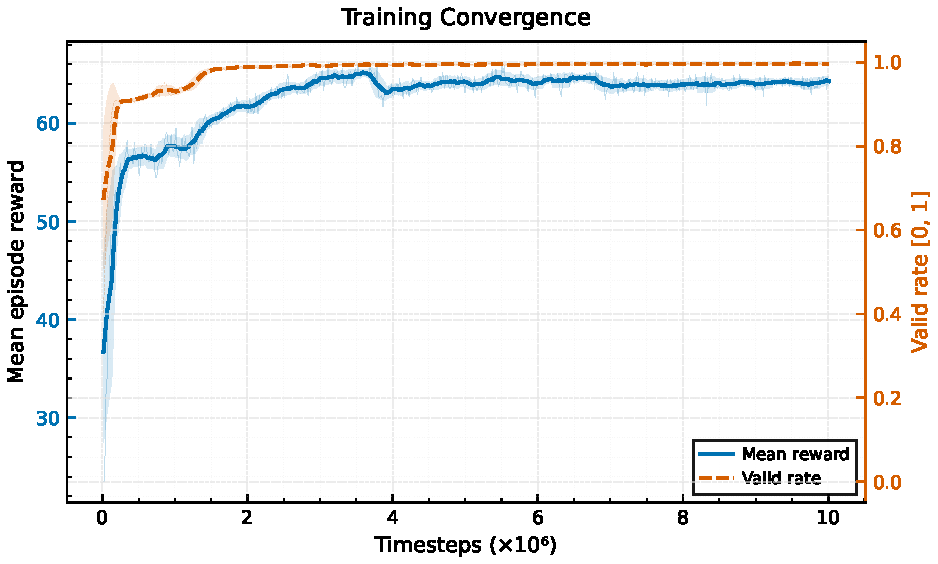
\includegraphics[width=0.8\textwidth]{images/chapter5/physics_informed/training_convergence.pdf}
        \caption{Mean episode reward and valid-action rate}
        \label{fig:physics_informed_training_convergence}
    \end{subfigure}
    
    \vspace{5pt}
    
    \begin{subfigure}{\textwidth}
        \centering
        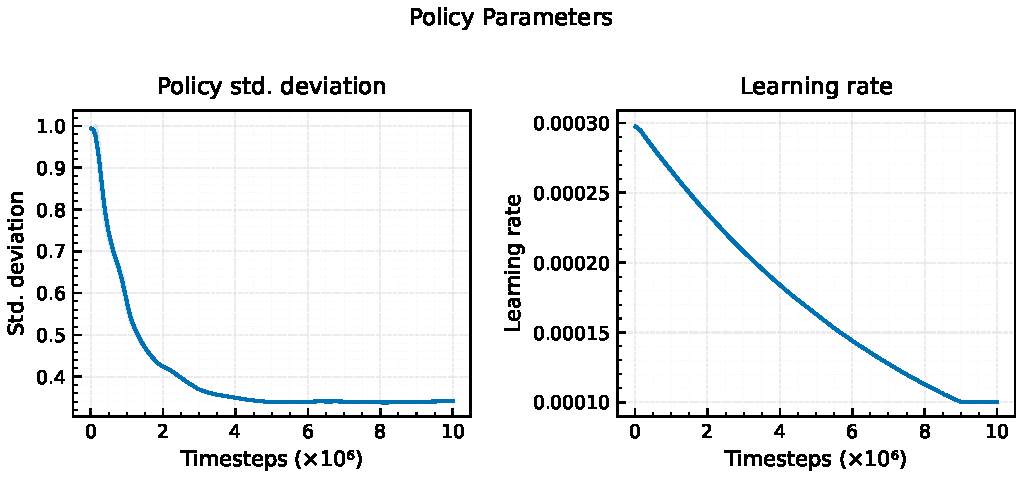
\includegraphics[width=0.8\textwidth]{images/chapter5/physics_informed/policy_parameters.pdf}
        \caption{Action standard deviation and learning rate}
        \label{fig:physics_informed_training_params}
    \end{subfigure}
    
    \vspace{5pt}
    
    \begin{subfigure}{\textwidth}
        \centering
        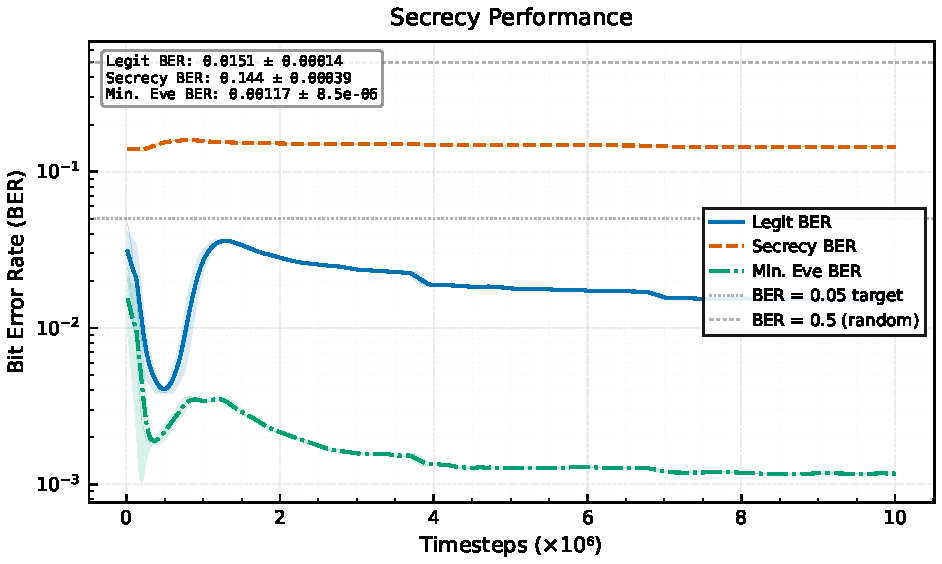
\includegraphics[width=0.8\textwidth]{images/chapter5/physics_informed/secrecy_performance.pdf}
        \caption{BER metrics (legitimate user, secrecy, and minimum eavesdropper)}
        \label{fig:physics_informed_training_ber}
    \end{subfigure}
    
    \caption{Training overview for the physics-informed action parameterisation}
    \label{fig:physics_informed_training}
\end{figure}

\begin{figure}[htbp]
    \centering
    \begin{minipage}[t]{0.49\textwidth}
        \centering
        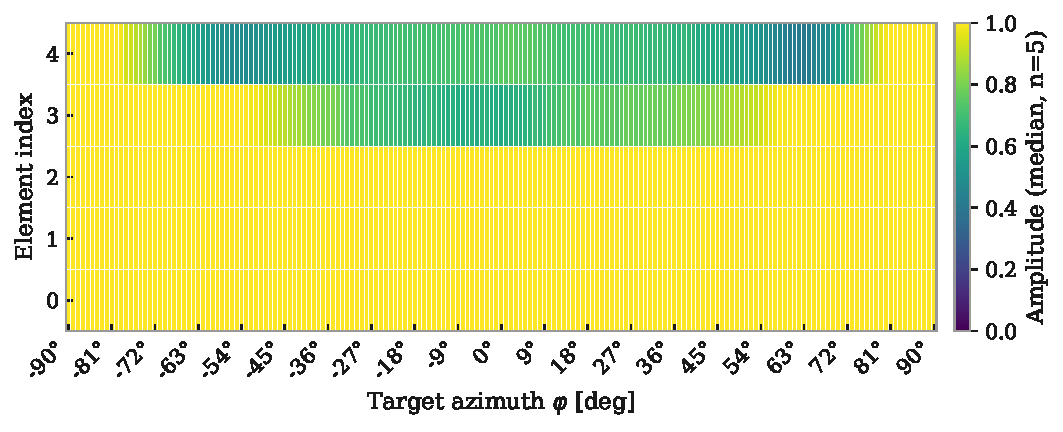
\includegraphics[width=\linewidth]{images/chapter5/physics_informed/amplitude_profile.pdf}
    \end{minipage}\hfill
    \begin{minipage}[t]{0.49\textwidth}
        \centering
        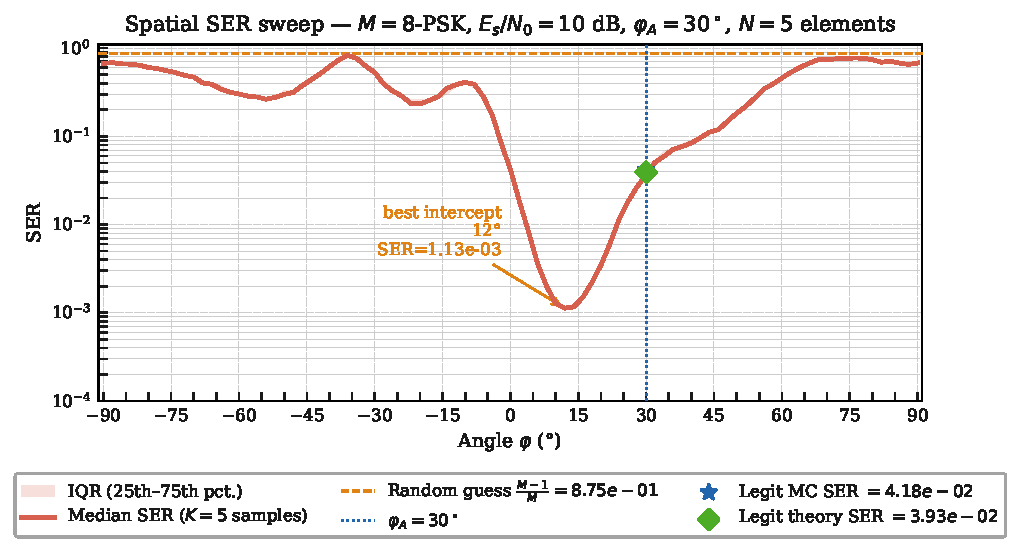
\includegraphics[width=\linewidth]{images/chapter5/physics_informed/ser_vs_angle.pdf}
    \end{minipage}\\[4pt]
    \begin{minipage}[t]{0.49\textwidth}
        \centering
        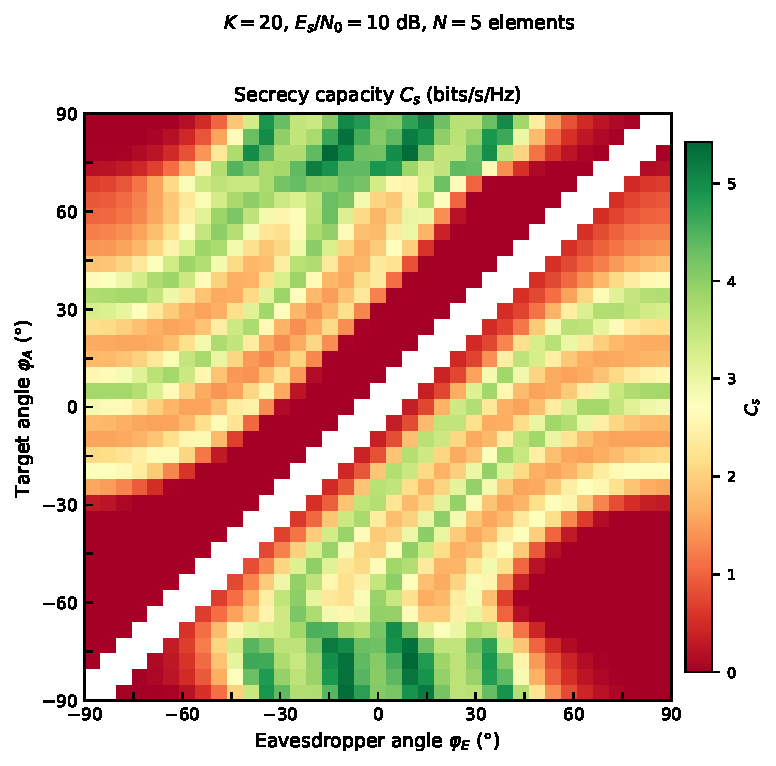
\includegraphics[width=\linewidth]{images/chapter5/physics_informed/secrecy_matrix.pdf}
    \end{minipage}\hfill
    \begin{minipage}[t]{0.49\textwidth}
        \centering
        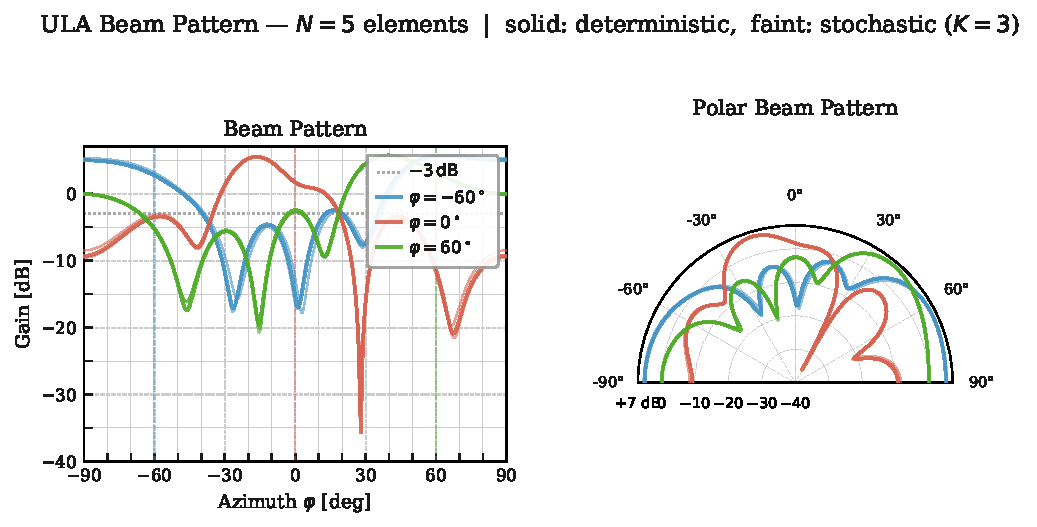
\includegraphics[width=\linewidth]{images/chapter5/physics_informed/beam_pattern.pdf}
    \end{minipage}
    \caption{Inference overview for the physics-informed action parameterisation. Top-left: amplitude profile across the full angular range. Top-right:\gls{BER} vs.\ azimuth angle at $E_s/N_0 = 10$\,dB with the legitimate user at $\varphi = 30\degree$. Bottom-left: secrecy matrix. Bottom-right: beam patterns for $\varphi \in \{-60\degree, 0\degree, 60\degree\}$.}
    \label{fig:physics_informed_inference}
\end{figure}

\begin{figure}[htbp]
    \centering
    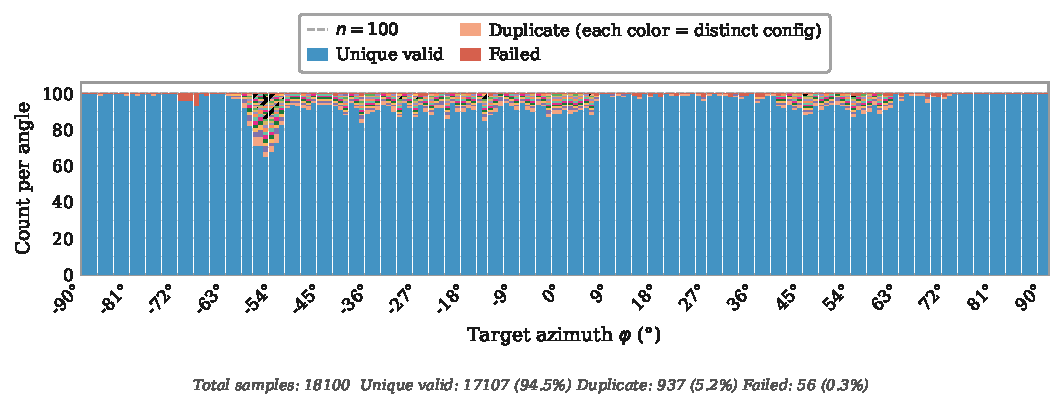
\includegraphics[width=1.0\textwidth]{images/chapter5/physics_informed/diversity_analysis.pdf}
    \caption{Outcome of 100 stochastic inference draws at each integer target angle $\varphi^* \in [-90\degree, 90\degree]$, for a total of 18{,}100 samples for the physics-informed action parameterisation. Each bar is decomposed into three categories: unique valid configurations (blue), duplicate solutions, and failed configurations that violated the amplitude or phase constraints (red).}
    \label{fig:diversity_analysis_physics_informed}
\end{figure}

\FloatBarrier

\subsection{ULA with \texorpdfstring{$N = 8$}{N = 8} elements}
\label{subsec:ula8}

Scaling from $N=5$ to $N=8$ elements introduces three compounding difficulties:
\begin{enumerate}
    \item the beamwidth narrows proportionally to $1/N$, so the fixed $\pm 5\degree$ validation window covers a larger fraction of the main lobe, making phase flatness harder to achieve;
    \item the action space grows to $2N=16$ dimensions, increasing the exploration burden and the credit-assignment difficulty per rollout;
    \item the phase of the normalised array response depends jointly on all $N$ element phases; with more elements, any inter-element misalignment produces stronger phase ripple across the support window.
\end{enumerate}
This experiment combines the physics-informed action parameterisation with a larger array, building on the results of \subsectionname~\ref{subsec:physics_informed}. All other hyperparameters, curriculum settings, and reward weights are identical to the $N=5$ baseline.

\figurename~\ref{fig:ula8_inference} and \figurename~\ref{fig:ula8_diversity_analysis} summarize the inference behavior, while \figurename~\ref{fig:ula8_training} summarizes the training dynamics.

\subsubsection{Results}
The experiment compounds the limitations identified in \subsectionname~\ref{subsec:physics_informed}. The inference results show that the physics-informed policy uses almost all elements at near-full amplitude, with at most one element slightly reduced, while the gradient-based baseline learns to silence or reduce elements. This root cause of this difference is that element silencing is only useful for\gls{DDM} secrecy when combined with non-ramp-like  phases; The gradient approach is free to pair reduced element amplitudes with unconventional phase assignments on the remaining elements, breaking the symmetry of the array response in a way that produces rapid phase variation outside the legitimate receiver's window. Under the physics-informed parameterisation, phases are constrained to stay within $\pm\frac{\pi}{4}$ of the\gls{DFT} ramp and silencing an element merely weakens and broadens the beam without generating the spatial phase variation that secrecy requires; The policy therefore correctly concludes that silencing is not worth the amplitude penalty since it gains nothing in secrecy. The diversity analysis (\figurename~\ref{fig:ula8_diversity_analysis}) shows that the duplicate rate is substantially higher than for $N=5$ and is distributed over the full angular range.

\begin{figure}[p]  % Force to its own page
    \centering
    \begin{subfigure}{\textwidth}
        \centering
        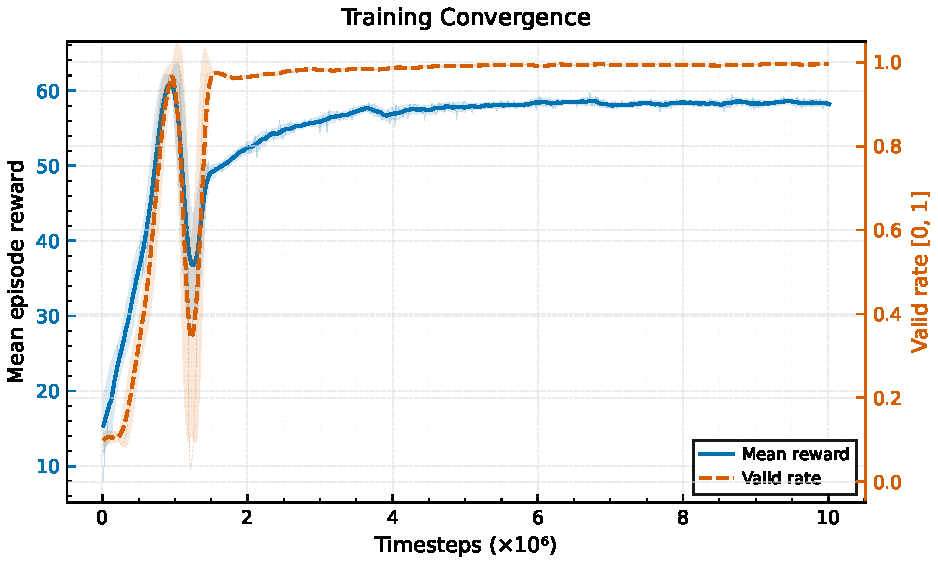
\includegraphics[width=0.8\textwidth]{images/chapter5/ula8/training_convergence.pdf}
        \caption{Mean episode reward and valid-action rate}
        \label{fig:ula8_training_convergence}
    \end{subfigure}
    
    \vspace{5pt}
    
    \begin{subfigure}{\textwidth}
        \centering
        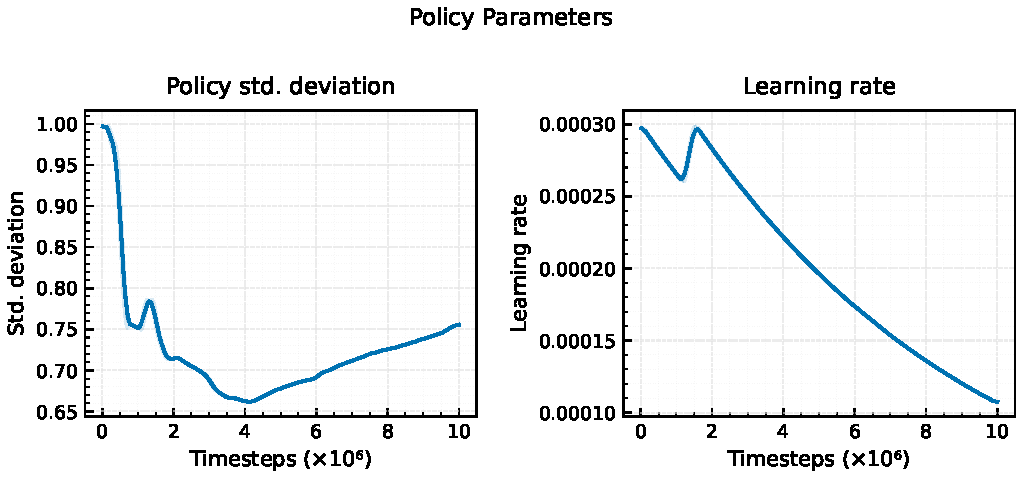
\includegraphics[width=0.8\textwidth]{images/chapter5/ula8/policy_parameters.pdf}
        \caption{Action standard deviation and learning rate}
        \label{fig:ula8_training_params}
    \end{subfigure}
    
    \vspace{5pt}
    
    \begin{subfigure}{\textwidth}
        \centering
        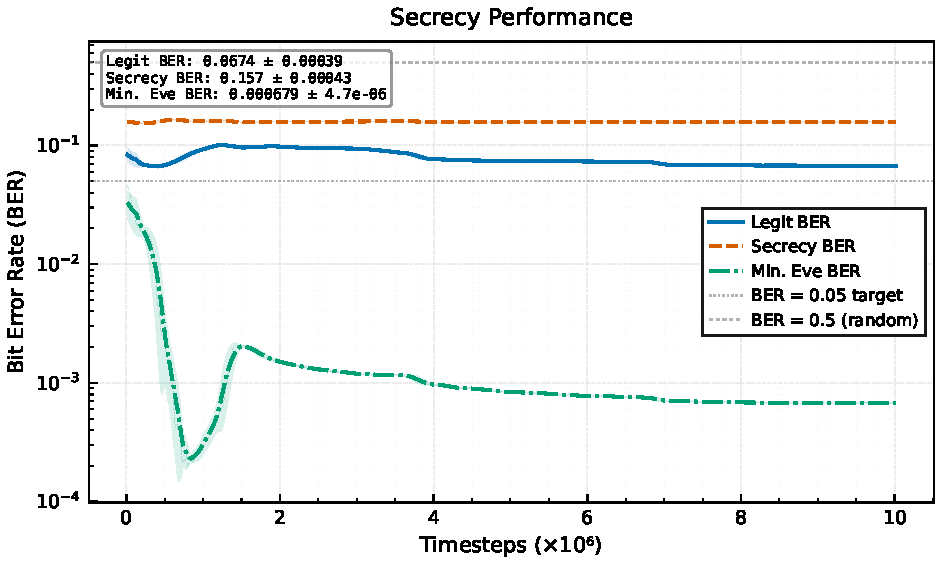
\includegraphics[width=0.8\textwidth]{images/chapter5/ula8/secrecy_performance.pdf}
        \caption{BER metrics (legitimate user, secrecy, and minimum eavesdropper)}
        \label{fig:ula8_training_ber}
    \end{subfigure}
    
    \caption{Training overview for the $N=8$\gls{ULA}. Top: mean episode reward and valid-action rate. Middle: action standard deviation and learning rate. Bottom:\gls{BER} metrics (legitimate user, secrecy, and minimum eavesdropper).}
    \label{fig:ula8_training}
\end{figure}

\begin{figure}[htbp]
    \centering
    \begin{minipage}[t]{0.49\textwidth}
        \centering
        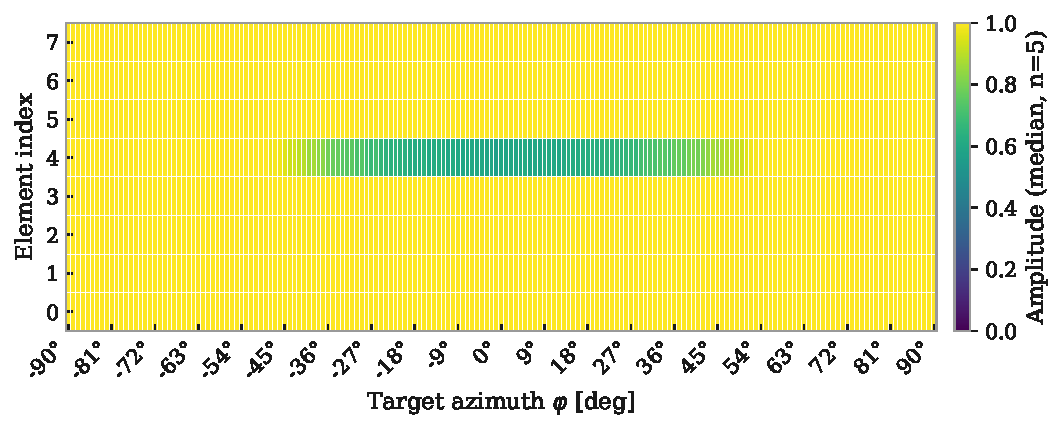
\includegraphics[width=\linewidth]{images/chapter5/ula8/amplitude_profile.pdf}
    \end{minipage}\hfill
    \begin{minipage}[t]{0.49\textwidth}
        \centering
        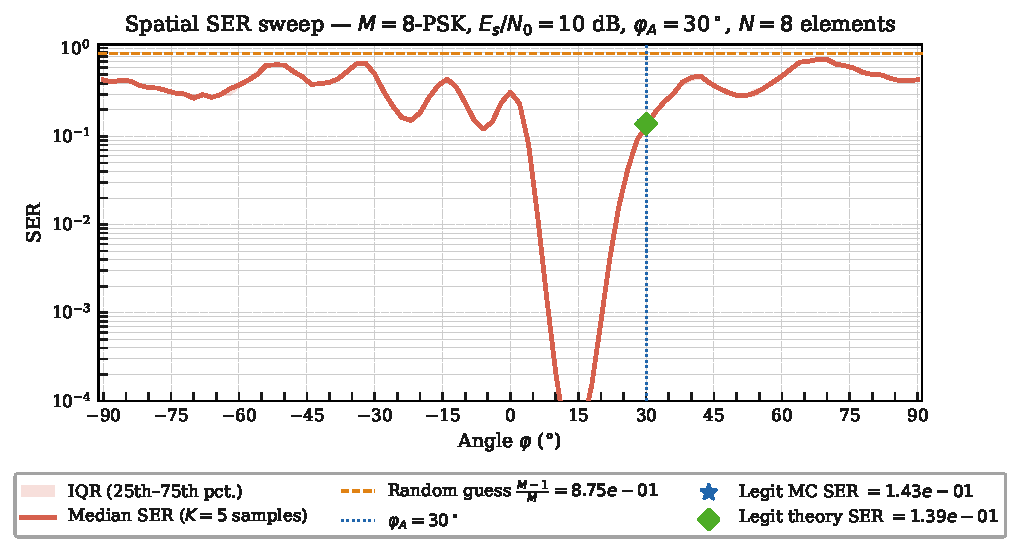
\includegraphics[width=\linewidth]{images/chapter5/ula8/ser_vs_angle.pdf}
    \end{minipage}\\[4pt]
    \begin{minipage}[t]{0.49\textwidth}
        \centering
        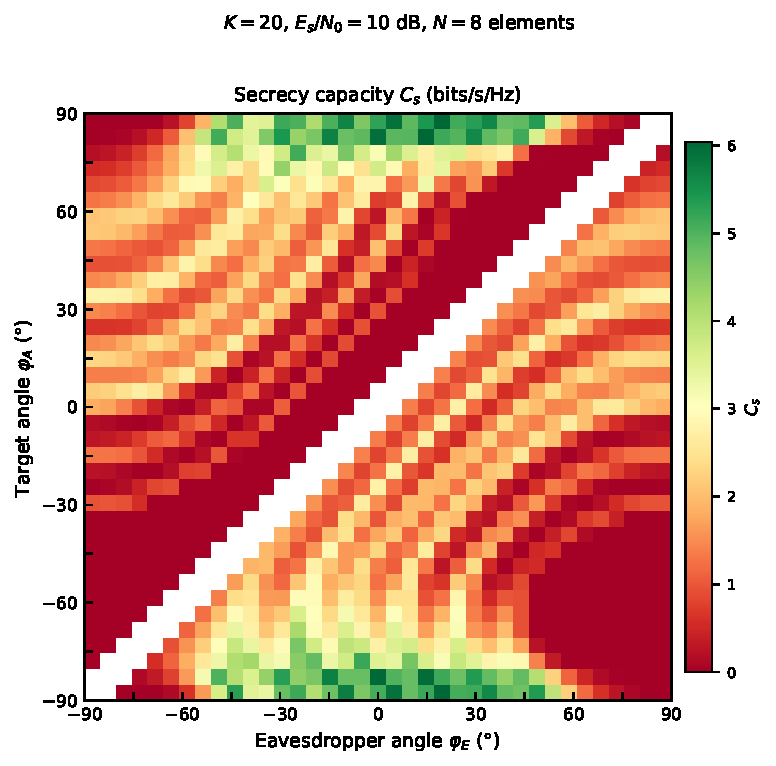
\includegraphics[width=\linewidth]{images/chapter5/ula8/secrecy_matrix.pdf}
    \end{minipage}\hfill
    \begin{minipage}[t]{0.49\textwidth}
        \centering
        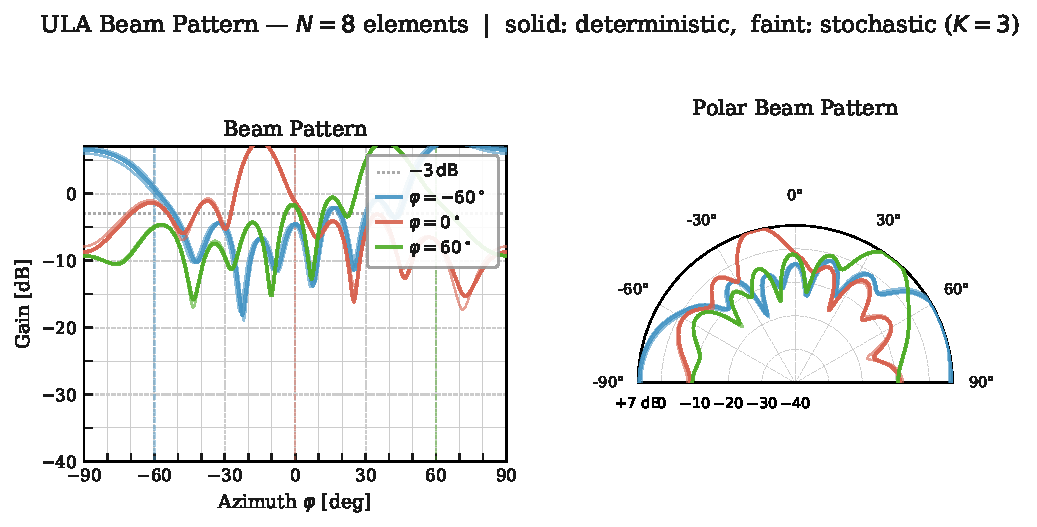
\includegraphics[width=\linewidth]{images/chapter5/ula8/beam_pattern.pdf}
    \end{minipage}
    \caption{Inference overview for the $N=8$\gls{ULA}. Top-left: amplitude profile across the full angular range.. Top-right:\gls{BER} vs.\ azimuth angle at $E_s/N_0 = 10$\,dB with the legitimate user at $\varphi = 30\degree$. Bottom-left: secrecy matrix. Bottom-right: beam patterns for $\varphi \in \{-60\degree, 0\degree, 60\degree\}$}
    \label{fig:ula8_inference}
\end{figure}

\begin{figure}[htbp]
    \centering
    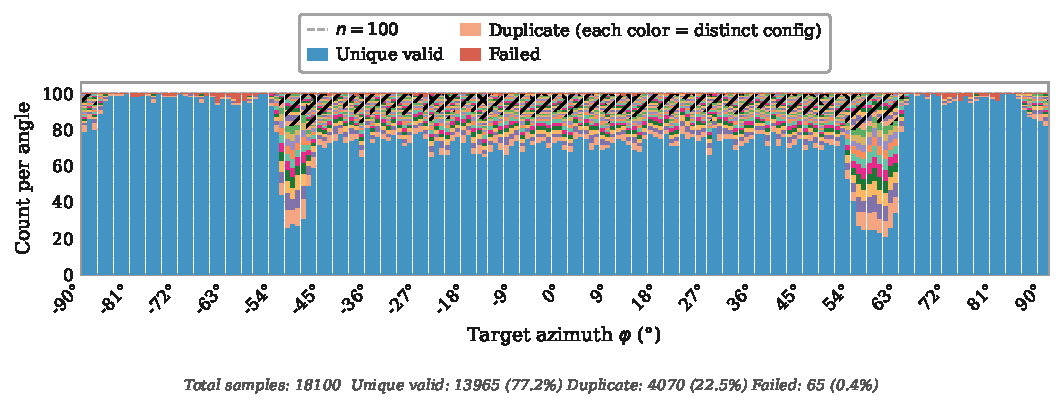
\includegraphics[width=1.0\textwidth]{images/chapter5/ula8/diversity_analysis.pdf}
    \caption{Outcome of 100 stochastic inference draws at each integer target angle $\varphi^* \in [-90\degree, 90\degree]$, for a total of 18{,}100 samples for the physics-informed action parameterisation with\gls{ULA} with $N=8$ elements. Each bar is decomposed into three categories: unique valid configurations (blue), duplicate solutions, and failed configurations that violated the amplitude or phase constraints (red).}
    \label{fig:ula8_diversity_analysis}
\end{figure}
\FloatBarrier